%% LaTeX2e class for student theses
%% sections/evaluation.tex
%% 
%% Karlsruhe Institute of Technology
%% Institute for Program Structures and Data Organization
%% Chair for Software Design and Quality (SDQ)
%%
%% Dr.-Ing. Erik Burger
%% burger@kit.edu
%%
%% Version 1.3, 2016-12-29

\chapter{Evaluation}
\label{ch:Evaluation}

This chapter is structured as follows: Initially the concept is elaborated (\autoref{sec:Evaluation:concept}), followed by evaluation scenarios (\autoref{sec:Evaluation:scenarios}) and the evaluation models (\autoref{sec:Evaluation:models}). The actual evaluation consists of the single tasks: monitoring (\autoref{sec:Evaluation:monitoring}), privacy analysis (\autoref{sec:Evaluation:monitoring}), model generation (\autoref{sec:Evaluation:privacyanalysis}) and system adaptation (\autoref{sec:Evaluation:planning}). Finally we are analysing the threats of validity (\autoref{sec:eval:threats}). Note, all evaluation models, test data and results can be found at \cite{privacy.PW}.

\section{Evaluation Design}
\label{sec:Evaluation:concept}

iObserve Privacy is a complex approach with many depending tasks. Evaluating the program as a whole is next to impossible due to the multiplexing dependencies. The evaluation factors would not be manageable and inconclusive results would make the evaluation itself pointless. So we decided to evaluate every task independently. The order and structure was inspired by the iObserve pipeline.

%Accuracy => Scenarios => unbiased
The task evaluation is generally split into an \textit{Accuracy} evaluation and a \textit{Scalability} evaluation. The accuracy evaluation aims for the correct functionality. This means, we are testing whether the actual results are equal to expected results. For the evaluation we are creating a set of \textit{Evaluation Scenarios}, which reflect real-world situations by defining a starting point and an expected endpoint. If the systems result differs from the endpoint, the reasons must be found and analysed.

%Scalability => Runtime behaviour, automatic generated PCMs, 1 > 10 > 100 > 1000 ... logarithmic scale
The scalability evaluation aims for the systems runtime characteristic, based on an increasing work load. The actual accuracy result of the task is of no interest during the analysis. The primary measurement is the tasks execution time, dependent on the assembly context count and resource container count. Both axis are logarithmic scaled, so the execution behaviour is clearly visible. The individual models are randomly generated, based on a repository model input.

We will use the \textit{Jaccard Coefficient} to evaluate model changes during the accuracy evaluation. Prior to the execution a target model is created, representing the desired post-execution state. The runtime model is compared to the target model, differences are calculated, as well as the jaccard coefficient. The coefficient is defined as the \textit{intersection set} of runtime and target model \textit{divided} through the \textit{union set} of these models:

$$JC(A,B)=\frac{\left | A \cap B \right |}{\left | A \cup B \right |}$$

If the models are completely equal, the result is \textit{1.0} \cite{Andale.20161202}. We are comparing the system model, the resource environment model and the allocation model. The repository and the usage model model is not modified by iObserve Privacy and therefore do not need any comparison. All models elements are matched by element content. The system and resource environment model are also compared by element ID. All models modified by iObserve Privacy are order independent, so an order match, like the \textit{Spearman Coefficient}, is not required.

The test device is a \textit{Surface Pro 4} using \textit{Windows 10} as Operating System. The important hardware specifications are a \textit{i7-6650U} processor with \textit{2.2 up to 3.4 GHz, 4 MB cache} and \textit{2 cores with hyper-threading}. The system uses 16 GB of RAM and a 265 GB Solid State Drive. For more details see \cite{Wikipedia.20170613}. The used \textit{Java} version is \textit{1.8.0\_121} form \textit{Oracle}.


\section{Evaluation Scenarios}
\label{sec:Evaluation:scenarios}

The scenarios are structured in \textit{PRE}, \textit{EVENT}, \textit{REACTION} and \textit{POST}. \textit{PRE} describes the distributed software system before the event takes place. The \textit{EVENT} is a trigger for a certain process or task chain, usually referenced as \textit{REACTION}. \textit{POST} defines the state of the software system after the reaction.

The scenarios describe the behaviour of iObserve Privacy through out all tasks, while each task gets evaluated individually. Nevertheless, details of a scenario may need clarification during the evaluation of this task.

The following scenarios are derived from the \textit{runtime changes} mentioned in \cite{Heinrich.2016b}. This runtime changes are possible modification to a distributed software system. However, not all mentioned scenarios are of interest in the privacy analysis context, these will be discussed in \autoref{eval:scenario:futile}. Scenarios 1 and 2 represent the observed system runtime changes, which trigger the iObserve privacy pipeline. These are designed to show the successful execution of a pipeline run with different triggers. Scenario 3 and 4 cover the \textit{operator-in-the-loop} scenarios. The operator is required, when an error occurs that iObserve privacy can not handle itself. These scenarios are design specific and therefore not derived from the runtime changes described in \cite{Heinrich.2016b}.

\subsection{Scenario 1: Default}
\label{eval:scenario:1}
% PRE: Amazon Deployment @ EU WEST
% CASE: Critical Error => Amazon moves instances to EU WEST & US EAST
% POST: Migration Monitored, Privacy Analysis started
%					=> IF OK:	Do nothing 
%					=> IF BAD:	Calculate Alternative (Privacy Compliant) => Plan => Adapt => Evaluate!
This scenario describes the "default" setting. It is used to evaluate the \textit{geo-location transformation}, the \textit{privacy analysis}, a successful execution of the \textit{re-deployment generation} and the \textit{adaptation planning}.

\begin{itemize}
	\setlength\itemsep{0em}
	\item \textbf{PRE}: All components of the software system are deployed on Amazons EC2 service on the \textit{EU Frankfurt} location. The system is privacy compliant.
	\item \textbf{EVENT}: Amazons EU Frankfurt data centre has a critical failure. As a result Amazon starts migrating local virtual machines towards the US Ohio and EU Ireland locations.
	\item \textbf{REACTION}: iObserve Privacy monitors the migration and starts a privacy analysis. The analysis shows a privacy violation and as a result an alternative, privacy compliant re-deployment is generated. A system adaptation plan is calculated based on the re-deployment and finally executed.
	\item \textbf{POST}: The software system is in a privacy compliant state.
\end{itemize}

\subsection{Scenario 2: System extension}
\label{eval:scenario:2}
% PRE: 	Privacy components @ Microsoft; Non-Privacy @ UKRAINE
% CASE:	New DePersonalized Component gets deployed @ UKRAINE
% POST: Deployment Monitored => Privacy Analysis started => "Joining Data Streams" found => Calculate Alternative (Privacy Compliant) => Plan => Adapt => Evaluate!

This scenario describes the deployment runtime change. It is used to evaluate the \textit{deployment transformation}, the \textit{privacy analysis}, a successful execution of the \textit{re-deployment generation} and the \textit{adaptation planning}.

%The deployment of a new software component triggers a privacy analysis, which detects "joining data streams" (see \autoref{sec:PrivacyAnalysis:theory}). This triggers the generation of an alternative deployment and the system adaptation. The pipeline works like in Scenario 1 without any operator interaction.
\begin{itemize}
	\setlength\itemsep{0em}
	\item \textbf{PRE}: All personal categorized components of the software system are deployed on Amazons EC2 service on the \textit{EU Frankfurt} location. All other components are hosted by an Ukrainian provider. The system is privacy compliant.
	\item \textbf{EVENT}: The system operator adds another component categorized as depersonalised to the Ukrainian server.
	\item \textbf{REACTION}: iObserve Privacy monitors the migration and starts a privacy analysis. The privacy analysis shows a privacy violation due to \textit{joining data streams}. An alternative, privacy compliant deployment is computed by PerOpteryx. A system adaptation plan is successfully calculated by the adaptation planning. Finally the adaptation sequence is executed.
	\item \textbf{POST}: The software system is in a privacy compliant state.
\end{itemize}

\subsection{Scenario 3: Failing Adaptation}
\label{eval:scenario:3}
% PRE: 	All @ Cheap Hoster (Europe SLA)
% CASE:	Some components migrate @ UKRAINE
% POST: Deployment Monitored => Privacy Analysis started => Privacy Violation found => Calculate Alternative (Privacy Compliant) => Plan => Adapt can't be done automatically => Call the Operator
This scenario is used to evaluate the \textit{operator-in-the-loop} during the \textit{execution} of the adaptation sequence. Due to at least one non-automated adaptation action the operator needs to be informed.

%The migration of a software component results in a privacy violating state. After the generation of a privacy compliant alternative and the calculation of the adaptation sequence, the operator is required. One or more adaptation actions can not be executed automatically. This is usually due to missing source control, like the \textit{Change Repository Component Action} or the \textit{Allocation Action}.
\begin{itemize}
	\setlength\itemsep{0em}
	\item \textbf{PRE}: All components of the software system are hosted by multiple server instances of a cloud reseller. 
	\item \textbf{EVENT}: The reseller migrates some of his servers to another cloud provider.
	\item \textbf{REACTION}: iObserve Privacy monitors the migration and starts a privacy analysis. The privacy analysis results in a privacy violation. An alternative privacy compliant deployment is computed. The adaptation calculation and planning is successful. The adaptation sequence contains actions that can not be executed automatically. The \textit{operator} is informed about the action that can not be executed by the \textit{adaptation execution}.
	\item \textbf{POST}: iObserve Privacy shows the operator the adaptation sequence with emphasis on the manual tasks.
\end{itemize}


\subsection{Scenario 4: Missing Alternative}
\label{eval:scenario:4}
% PRE: 	All @ Cheap Hoster (Europe SLA)
% CASE:	Some components migrate @ UKRAINE
% POST: Deployment Monitored => Privacy Analysis started => Privacy Violation found => Calculate Alternative (Privacy Compliant) => No Privacy Compliant Alternative Found => Call Operator

This scenario is used to evaluate the \textit{operator-in-the-loop} during the \textit{re-deployment generation}. PerOpteryx did not provide a privacy compliant re-deployment model and therefore the operator is notified.

%This scenario describes the use case, where no privacy compliant, alternative deployment could be calculated. The migration of a software components results in a privacy violating state. The calculation of privacy compliant alternatives deployment fails. The operator needs to be informed about the current situation.
\begin{itemize}
	\setlength\itemsep{0em}
	\item \textbf{PRE}: All components of the software system are hosted by multiple server instances of a cloud resellers. 
	\item \textbf{EVENT}: The reseller starts migrating his servers to another cloud provider.
	\item \textbf{REACTION}: iObserve Privacy monitors the migration and starts a privacy analysis. The privacy analysis shows a privacy violation. The computation of an alternative privacy compliant deployment fails. iObserver privacy detects that the re-deployment model is missing or not privacy compliant. The \textit{operator} is notified about the situation.
	\item \textbf{POST}: iObserve Privacy notifies the operator about the missing privacy compliant re-deployment model.
\end{itemize}

%\subsection{Scenario 5}
% PRE: 	Privacy components @ Amazone EU WEST; Non-Privacy @ Cheap Hoster (Europe SLA)
% CASE:	Cheap Hoster constantly migrates to the cheapest hoster => Moves two Depersonal instances to the same server in Ukraine
% POST: Migration Monitored, Privacy Analysis started
%			=> "Joining Data Streams" found => Calculate Alternative (Privacy Compliant) => Plan => Adapt => Evaluate!

\subsection{Futile Scenario}
\label{eval:scenario:futile}
There are a couple of scenarios which do not apply to iObserve Privacy, due to various reasons \cite{Heinrich.2016b}. We will elaborate those scenarios shortly.

%Performance
Performance or workload characteristics are not tackled, since performance and privacy analysis combined wouldn't be manageable in the scope of this thesis.

%Undeployment
The un-deployment or de-replication are two scenarios which reduce the complexity of the privacy analysis. A privacy violation can not be triggered by eliminating a component and/or a server from the system.

%Replication
The replication of a server, with all its components, will trigger a deployment event. This means, this scenario is already covered by \textit{Scenario 2}.


\section{Evaluation Models}
\label{sec:Evaluation:models}

In the previous sections we defined a couple of scenarios for the evaluation. In order to execute these scenarios, we need PCM Privacy models (\autoref{ch:pcmExtension}). Scenario and model need to get selected individually, depending on the task to evaluate.

\subsection{CoCoME-Cloud}
\label{sec:eval:models:cocome}

The \textit{CoCoME Cloud} PCM model is a representation of the CoCoME system as a distributed cloud variant. It is a representation of a supermarket IT infrastructure. It consists of six individual deployed components:  \textit{logic.webservice.cashdeskline.cashdeskservice}, \textit{cloud.web}, \textit{traidingsystem.inventory}, \textit{traidingsystem.cashdeskline}, \textit{webservice.inventory} and \textit{traidingsystem.external.bank}. The system design is oriented on real distributed software systems with dozens of interfaces and multiple composite components. As a result, CoCoME-Cloud is very complex and not suited for the evaluation of specific aspects like the component categorization or the deployment analysis. However, it is as the only available model fully specified and "PerOpteryx ready". See \cite{Heinrich.2015} for detailed information on CoCoME.


\subsection{Medi System}
\label{sec:eval:models:medSys}

\begin{figure}[h]
	\centering
	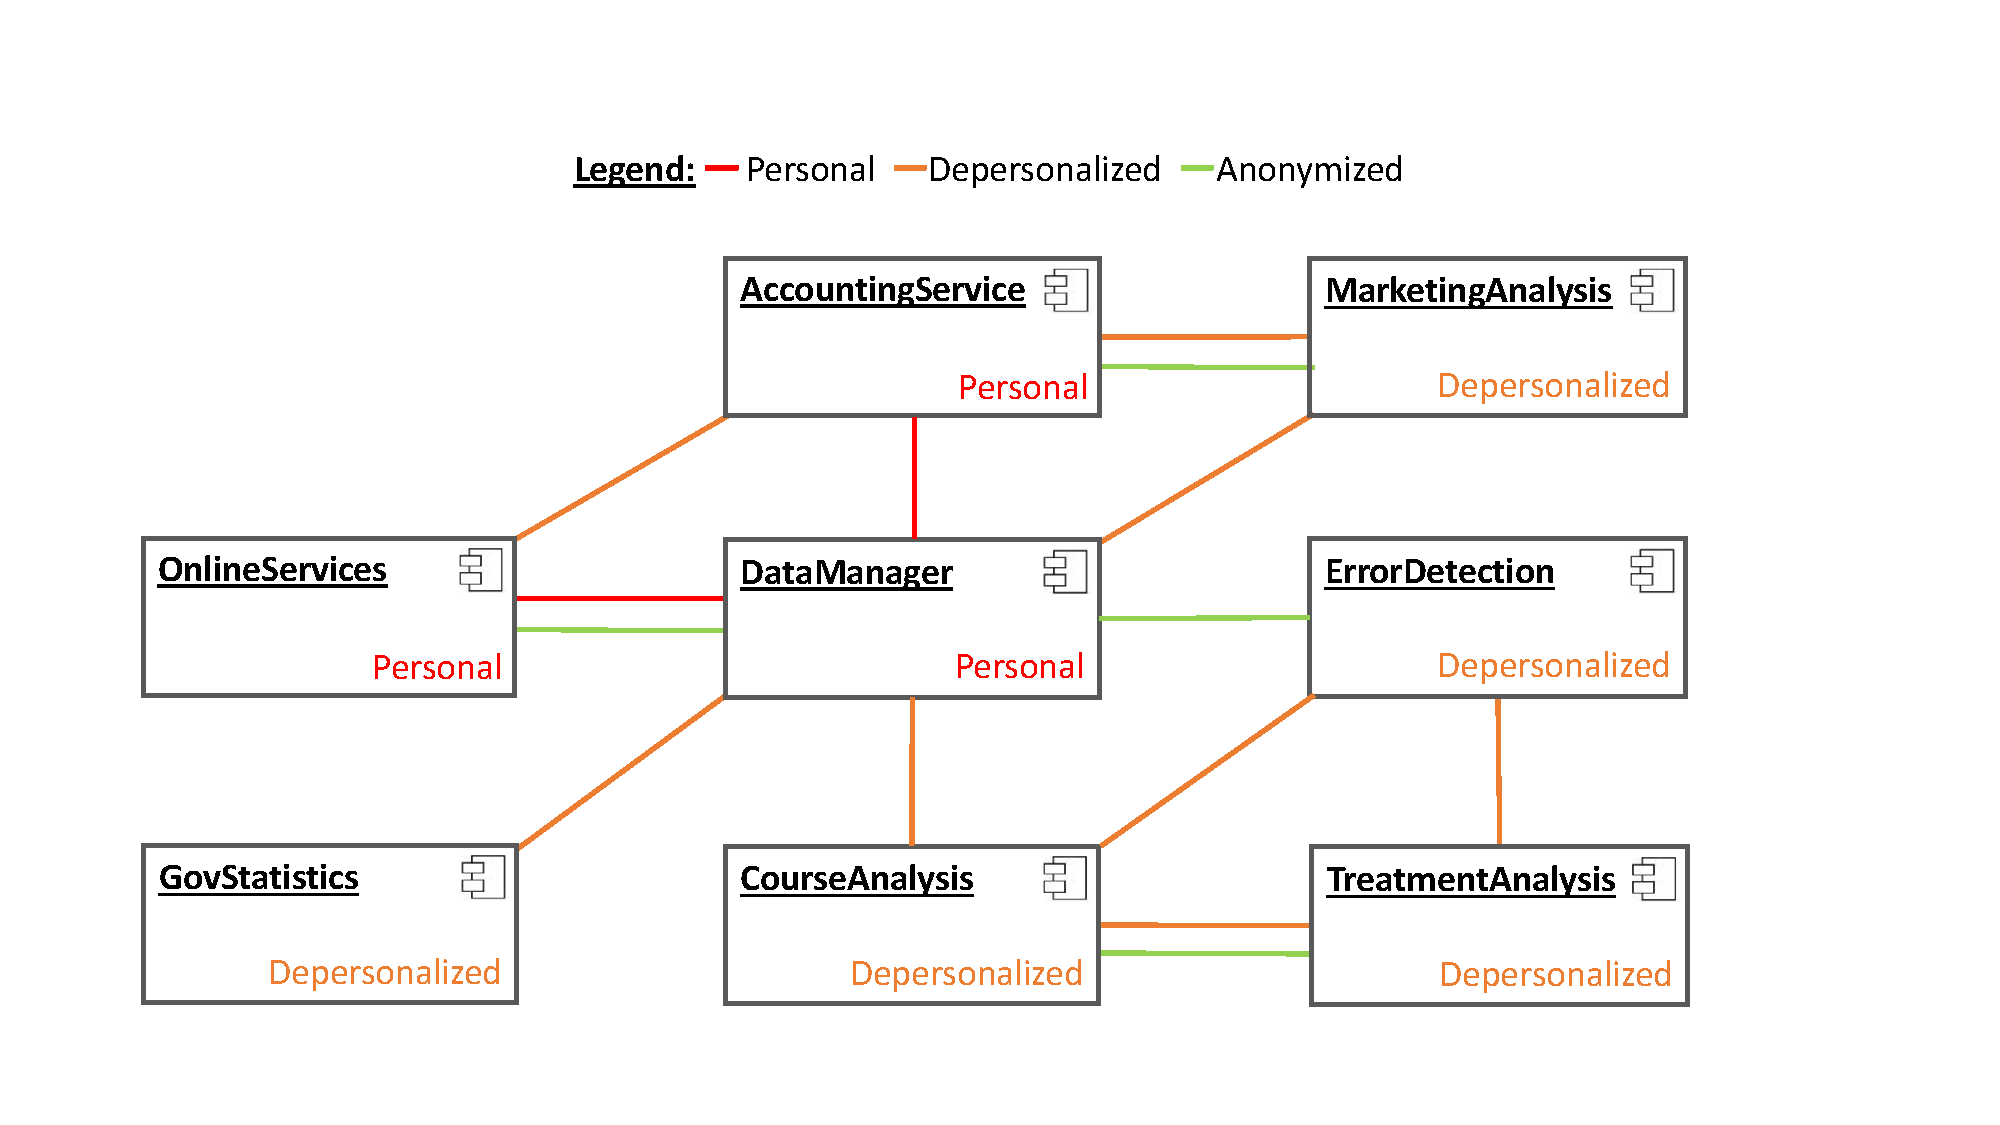
\includegraphics[trim = 0mm 10mm 0mm 20mm, clip, width=0.90\textwidth]{graphs/medSystem_noserver}
	\caption{Initial component categorization}
	\label{fig:model:medi}
\end{figure}

The \textit{Medi System} is an PCM model, specially developed for the evaluation of this thesis. It is supposed to reflect the web system of a medical insurance. The required and provided interfaces are reduced to the minimal necessity, to limit side effects and to gain meaningful results. \autoref{fig:model:medi} shows the medi system with all components and interface connections. The deployment will depend on the evaluation scenario.


\subsection{Generated Models}
\label{sec:Evaluation:models:generated}

We developed a model generator and model modificator for the scalability analysis. The generator requires an input repository and creates a valid PCM Privacy model with the given amount of assembly contexts and resource containers. The contained component in the assembly context is randomly selected, as well as the resource container it is allocated on. All required interfaces are correctly connected, primarily to provided interfaces without an existing connection.

The model is usually constructed with a distribution of 40\% Resource Container and 60\% Assembly Contexts. This means, a model with 1000 nodes consists of 400 servers and connected 600 components. We argue, that this leads to a near real-world distribution of servers with the majority of servers hosting one or two components, a few hosting three or more components and some empty servers. The classification of the Assembly Connectors is distributed among 15\% Personal, 35\% Depersonalised and 50\% Anonymous. This distribution is oriented on the \textit{CoCoME} classification.

The combination of node and classification distribution leads to every possible execution path during the execution, as tests have shown. This is the primary concern for the scalability tests, since the tests aim for a near real-world setting.

The model modificator adapts the system randomly, based on action counts specified. The modification supports server acquisition and termination and assembly context allocation, deallocation and migration. Further, it supports the exchange of the contained repository component for a component with the same interfaces. Note, the generated models are only suited for the scalability analysis. 



\section{Transformation}
\label{sec:Evaluation:monitoring}

The Transformation evaluation consists of an accuracy and a scalability evaluation. The main purpose is to test the transformation of the sent information to the architectural runtime model. Further, the iObserve privacy pipeline has to be triggered upon changes. \textit{Scenario \#1} (\autoref{eval:scenario:1}) and \textit{Scenario \#2} (\autoref{eval:scenario:2}) describe the two possible triggers: the \textit{Deployment Event}, when a component is deployed on a server, and the \textit{GeoLocation Event}, when the geo-location of a server changes. 

\subsection{Transformation: Accuracy Evaluation}

For the accuracy evaluation we are using the CoCoME-Cloud model (\autoref{sec:eval:models:cocome}), since it is completely specified and reflects a real-world system the most appropriate way available. We need to show, that the TDeployment, TUndeployment and TGeoLocation Transformations apply the sent data correctly to the PCM model. Potential errors must be handled and processed. For this purpose we will use two executions. First, we will execute a logically valid input set of events, to show the correctness of the transformation. In a second execution we will show, that logically wrong inputs are processed correctly. Both runs start with an empty allocation model.

\autoref{tab:valid_run} shows the initial input event sequence. Initially all components are being deployed, followed by a geo-location update for each server and a re-deployment of the \textit{cloud.web} component from \textit{Server1-EU} to \textit{Server5-EU} and finally a geo-location update on \textit{Server4-EU} to Ukraine.

\begin{table}[h]
	\centering
	\begin{tabular}{r | l}
		\hline
		\textbf{Action} & \textbf{Values}\\
		\hline
		Deployment & tradingsystem.external.Bank on Server6-EU\\
		Deployment & tradingsystem.cashdeskline on Server4-EU\\
		Deployment & cloud.web on Server1-EU\\
		Deployment & webservice.inventory on Server1-EU\\
		Deployment & tradingsystem.inventory on Server2-EU\\
		Deployment & logic.webservice.cashdeskline.cashdeskservice on Server3-EU\\
		GeoLocation & Server1-EU on 276 (GER)\\
		GeoLocation & Server2-EU on 276 (GER)\\
		GeoLocation & Server3-EU on 250 (FRA)\\
		GeoLocation & Server4-EU on 250 (FRA)\\
		GeoLocation & Server5-EU on 826 (GBR)\\
		GeoLocation & Server6-EU on 826 (GBR)\\
		UnDeployment & cloud.web from Server1-EU\\
		Deployment & cloud.web on Server5-EU\\
		GeoLocation & Server4-EU on 804 (UKR)\\
		\hline
		\end{tabular}
	\caption{The correct execution set}
	\label{tab:valid_run}
\end{table}

We expect a run without any errors, an allocation model, which represents the described deployment and a design decisions model, with the according degree of freedoms.

The results are true to our expectations. The system reports no errors and the models represent the system exactly as intended. The \textit{Jaccard Coefficient} is \textit{1.0}.

\begin{table}[h]
	\centering
	\begin{tabular}{r | l}
		\hline
		\textbf{Action} & \textbf{Values}\\
		\hline
		\multicolumn{2}{ c }{\autoref{tab:valid_run} commands}\\
		Deployment & cloud.web on Server1-EU*\\
		UnDeployment & cloud.web from Server5-EU\\
		UnDeployment & cloud.web from Server5-EU*\\
		Deployment & cloud.web on Server7-EU*\\
		Deployment & IllegalComonent on Server1-EU*\\
		UnDeployment & IllegalComonent from Server1-EU*\\
		UnDeployment & tradingsystem.inventory from Server3-EU*\\
		GeoLocation & Server7-EU on 826 (GBR)*\\
		\hline
	\end{tabular}
	\caption{The error execution set}
	\label{tab:error_run}
\end{table}

To test the error behaviour, we need to input logically false events. To gain a valid system state, we are starting with the valid order (\autoref{tab:valid_run}) and append illegal orders. \autoref{tab:error_run} shows the exact execution sequence. Illegal events are marked with a *. We expect these orders to give a warning and to be ignored. The system must continue running. The test includes the following cases: Deployment of an already deployed component, deployment or undeployed on a non-existing server, geo-location record from a non-existing server, un-deployment of a non-existing deployment.


The error run ends up to be exactly as intended. All faulty commands got ignored and the \textit{Jaccard Coefficient} is \textit{1.0}. Both Jaccard coefficients show, that the (un-)deployment and geo-location transformation works as anticipated. As a consequence we argue, that the \textit{monitoring} research question, \textbf{RQ-M1}, was successfully answered and that we have a very good accuracy (see \textbf{RQ-M2}), since no case could be identified that did not work as intended.


\subsection{Transformation: Scalability Evaluation}

For the scalability analysis we are using the Medi-System model with generated input. The Medi-Model is chosen due to its less generic characteristic then the Gen-Model and therefore more realistic result. Further, the Medi-Model as complex as the CoCoME model in the field to test, while easier to understand and less error prone during input generation.

The inputs are logically and syntactically valid. 30\% of the inputs are deployments and un-deployments, distributed relative to the current allocation status. The other 70\% of inputs are geo-location events, randomly distributed over all available servers. This ratio is an over-approximation towards the more complex and computation intensive allocation and de-allocation events. The expected real-world occurrence of a deployment events to the geo-location event is about 1 to 10000. This way, we expect the deployment and un-deployment event to have a more significant impact on the runtime behaviour. Every measurement was repeated ten times to eliminate potential measurement errors. The log outputs remain active, the snapshot creation is deactivated, so no further pipeline filters are activated. We use input sizes from 10 to one million events on a logarithmic scale.

\begin{figure}[h]
	\centering
	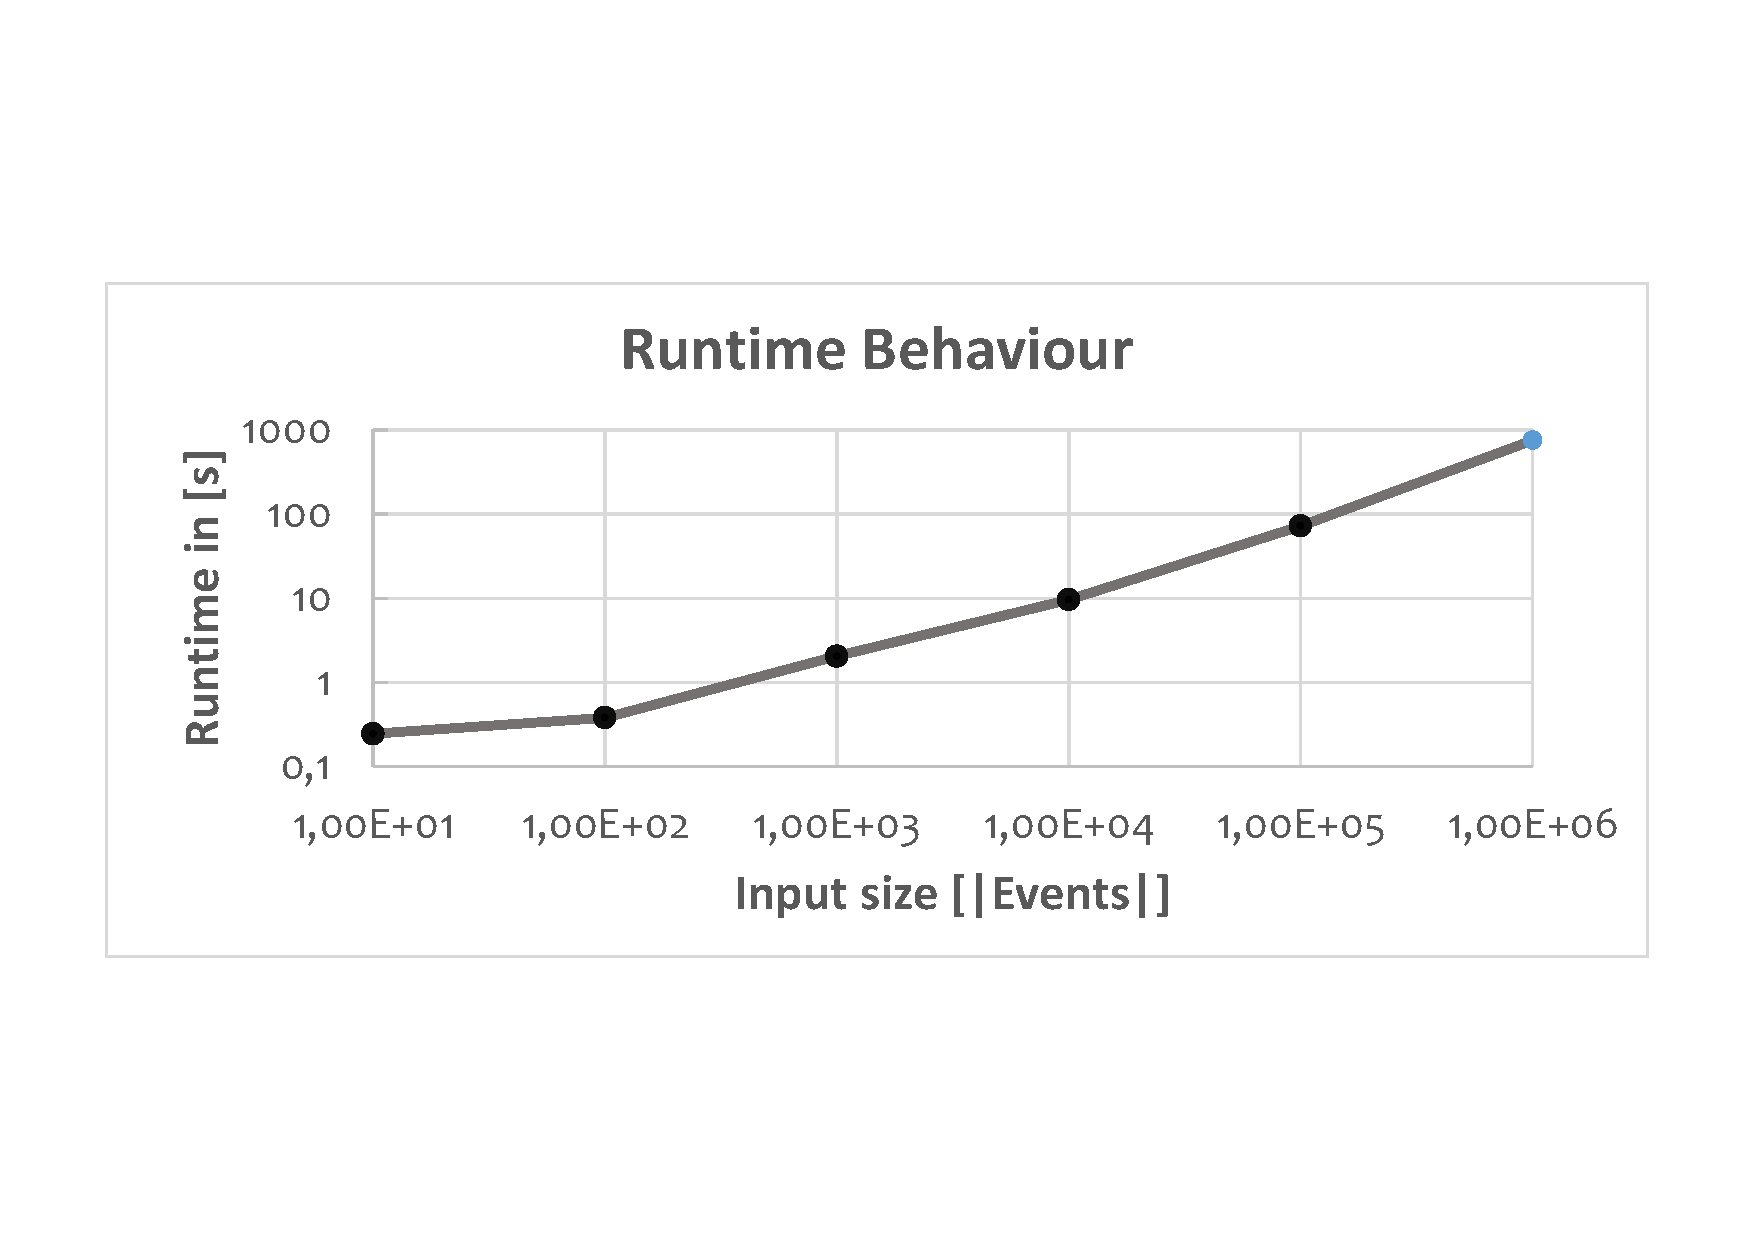
\includegraphics[trim = 10mm 90mm 10mm 110mm, clip, width=0.90\textwidth]{graphs/Runtime_Transformation}
	\caption{Transformation runtime \& Standard Deviation}
	\label{fig:eval:trans:runtime}
\end{figure}

The results (\autoref{fig:eval:trans:runtime}) show a linear runtime behaviour, for the maximum input size of 1 million events the execution takes about 820 seconds. The according standard deviation of 22 makes it a stable and fast result, concerning \textbf{RQ-M3}.

\section{Privacy Analysis}
\label{sec:Evaluation:privacyanalysis}

The \textit{Privacy Analysis} was discussed in \autoref{ch:PrivacyConcept} (Privacy Concept) and \autoref{ch:PrivacyAnalysis} (Privacy Analysis). As described there, the privacy analysis consists of two sequential parts: \textit{Component Classification} and \textit{Deployment Analysis}. According to this tasks, the accuracy evaluation is also split. The accuracy evaluation uses the Medi-System model (\autoref{sec:eval:models:medSys}), due to its moderate complexity level, where effects like the \textit{Joining Data Stream} occur, but the results are still traceable.

\subsection{Privacy Analysis: Accuracy Evaluation}

We will show, that the \textit{Component Classification} categorizes components correctly. This includes the correct initial categorization $(C1)$, the finding of \textit{joining data streams} $(C2)$ and \textit{single data stream} $(C3)$. Further, we will show, that the \textit{Deployment Analysis} finds illegally deployed personal components on un-save geo-locations $(D1)$, \textit{joining data streams} on the deployment level $(D2)$ and ignores \textit{joining data streams} on a save geo-location $(D3)$. As a result, we demonstrate the correctness of our privacy analysis, as specified in the goal section (\autoref{sec:Introduction:goals}).

The scenarios \#1 (\autoref{eval:scenario:1}) and \#2 (\autoref{eval:scenario:1}) aim to trigger a privacy analysis and describe different privacy violations. We showed in \autoref{sec:Evaluation:monitoring}, that both trigger, the deployment event and the geo-location event are correctly processed and the information, are successfully transformed to the PCM model. Both pipeline triggers lead to the same privacy analysis and are therefore equivalent for this accuracy evaluation. 

% Effects to show
% Categorization: Initial Categorization + JDS + Single DS
% Deployment Analysis: Personal on un-save Server + JDS on un-save Server + JDS on save Server

\begin{figure}[h]
	\centering
	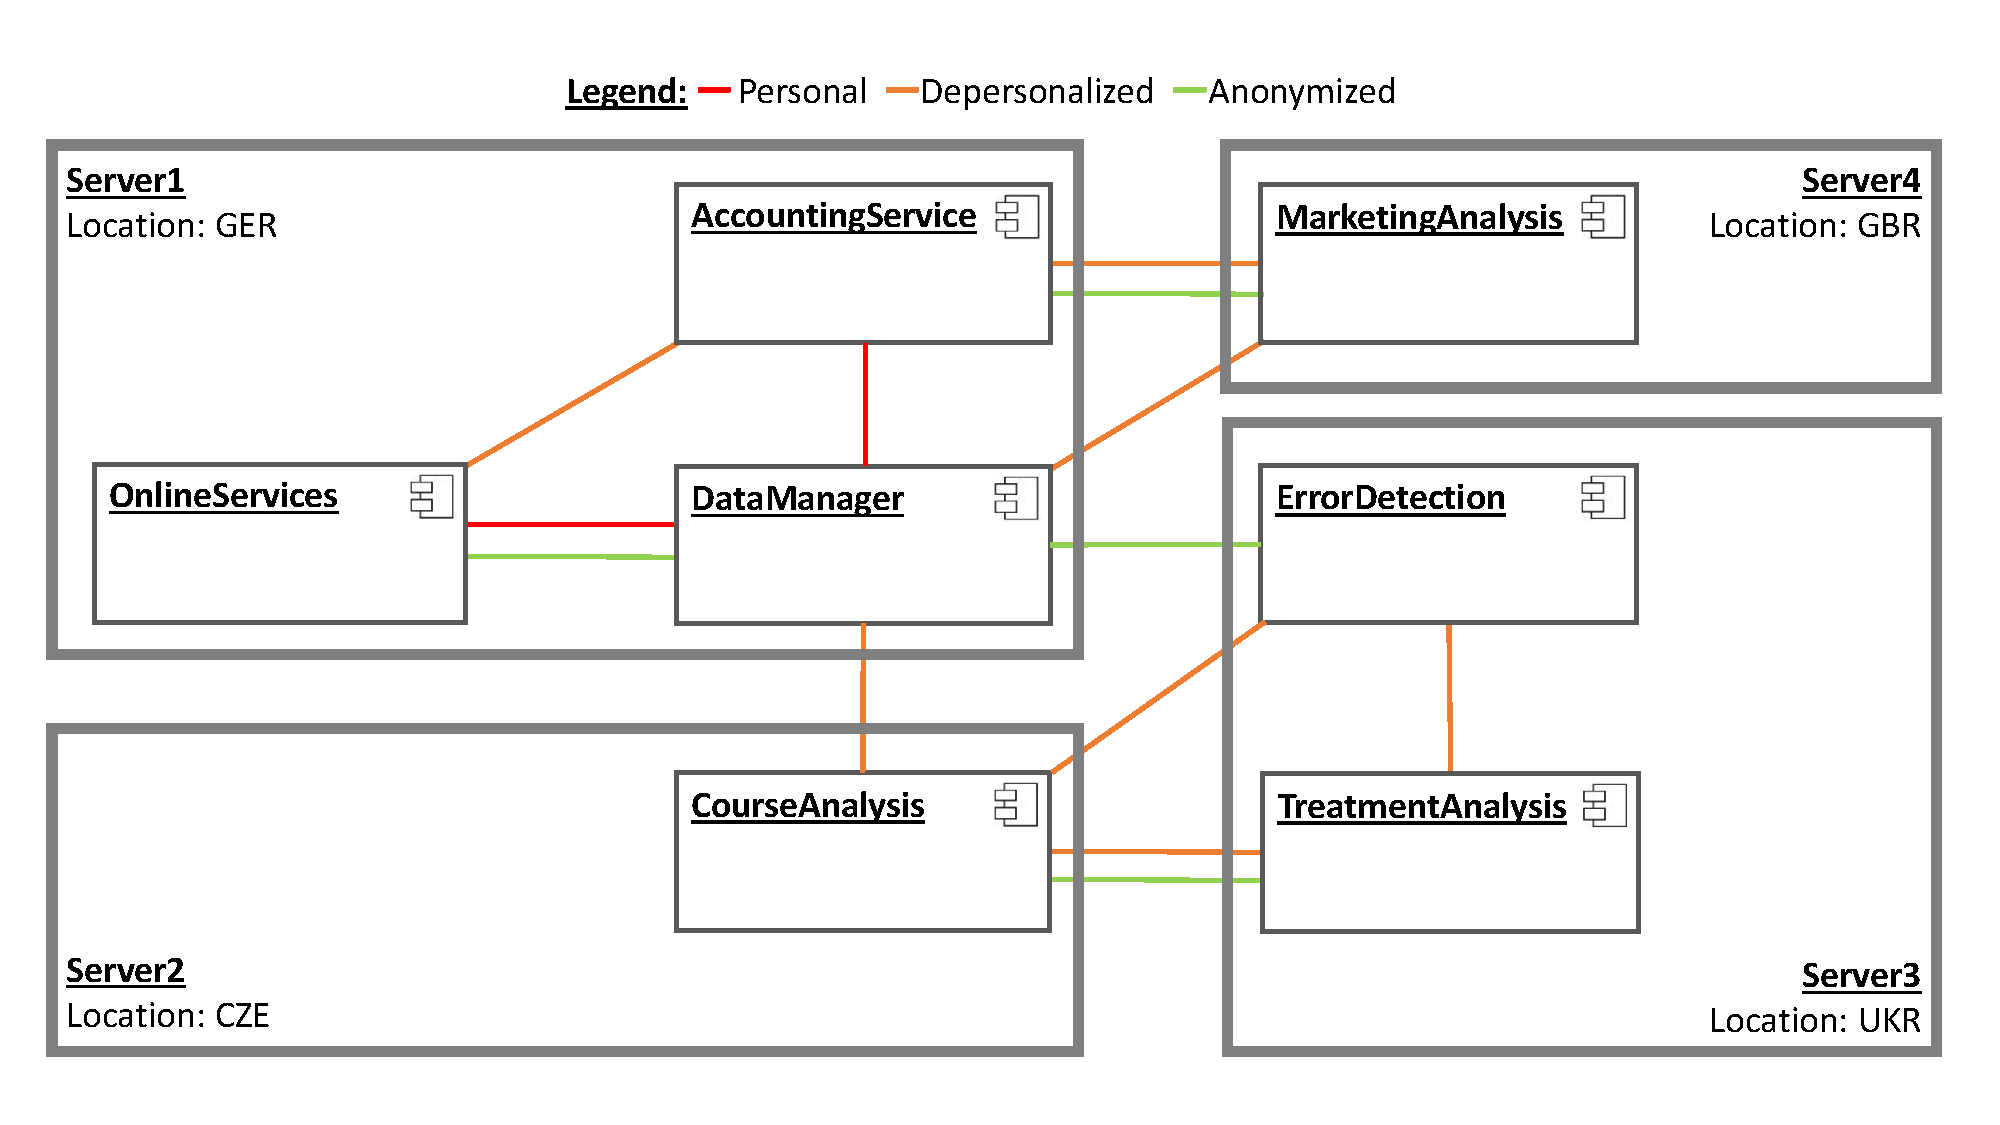
\includegraphics[trim = 0mm 10mm 0mm 10mm, clip, width=0.75\textwidth]{graphs/medSys_eval_pa_init}
	\caption{Initial system state}
	\label{fig:eval:pa:init}
\end{figure}

The initial system state is as shown in \autoref{fig:eval:pa:init}. The system is privacy compliant and only the \textit{GovStatistics} component is not allocated on a server. iObserve will trigger the pipeline by processing a TGeoLocation transformation, which migrates the \textit{Server2} to Belarus. With this trigger, we will show, that the component categorization works as intended.

We expect the initial component categorization to be equal to the most personal interface level the component has $(C1)$. After the \textit{Categorization Analysis} the \textit{MarketingAnalysis} component should be classified as personal, due to its two personal communication partners $(C2)$. The privacy level categorization of the components \textit{ErrorDetection}, \textit{TreatmentAnalysis} and \textit{CourseAnalysis} must remain unchanged, since they share a single depersonalised interface as data source $(C3)$. The deployment must remain legal.

\begin{figure}[h]
	\centering
	\begin{minipage}[b]{0.48\textwidth}		
		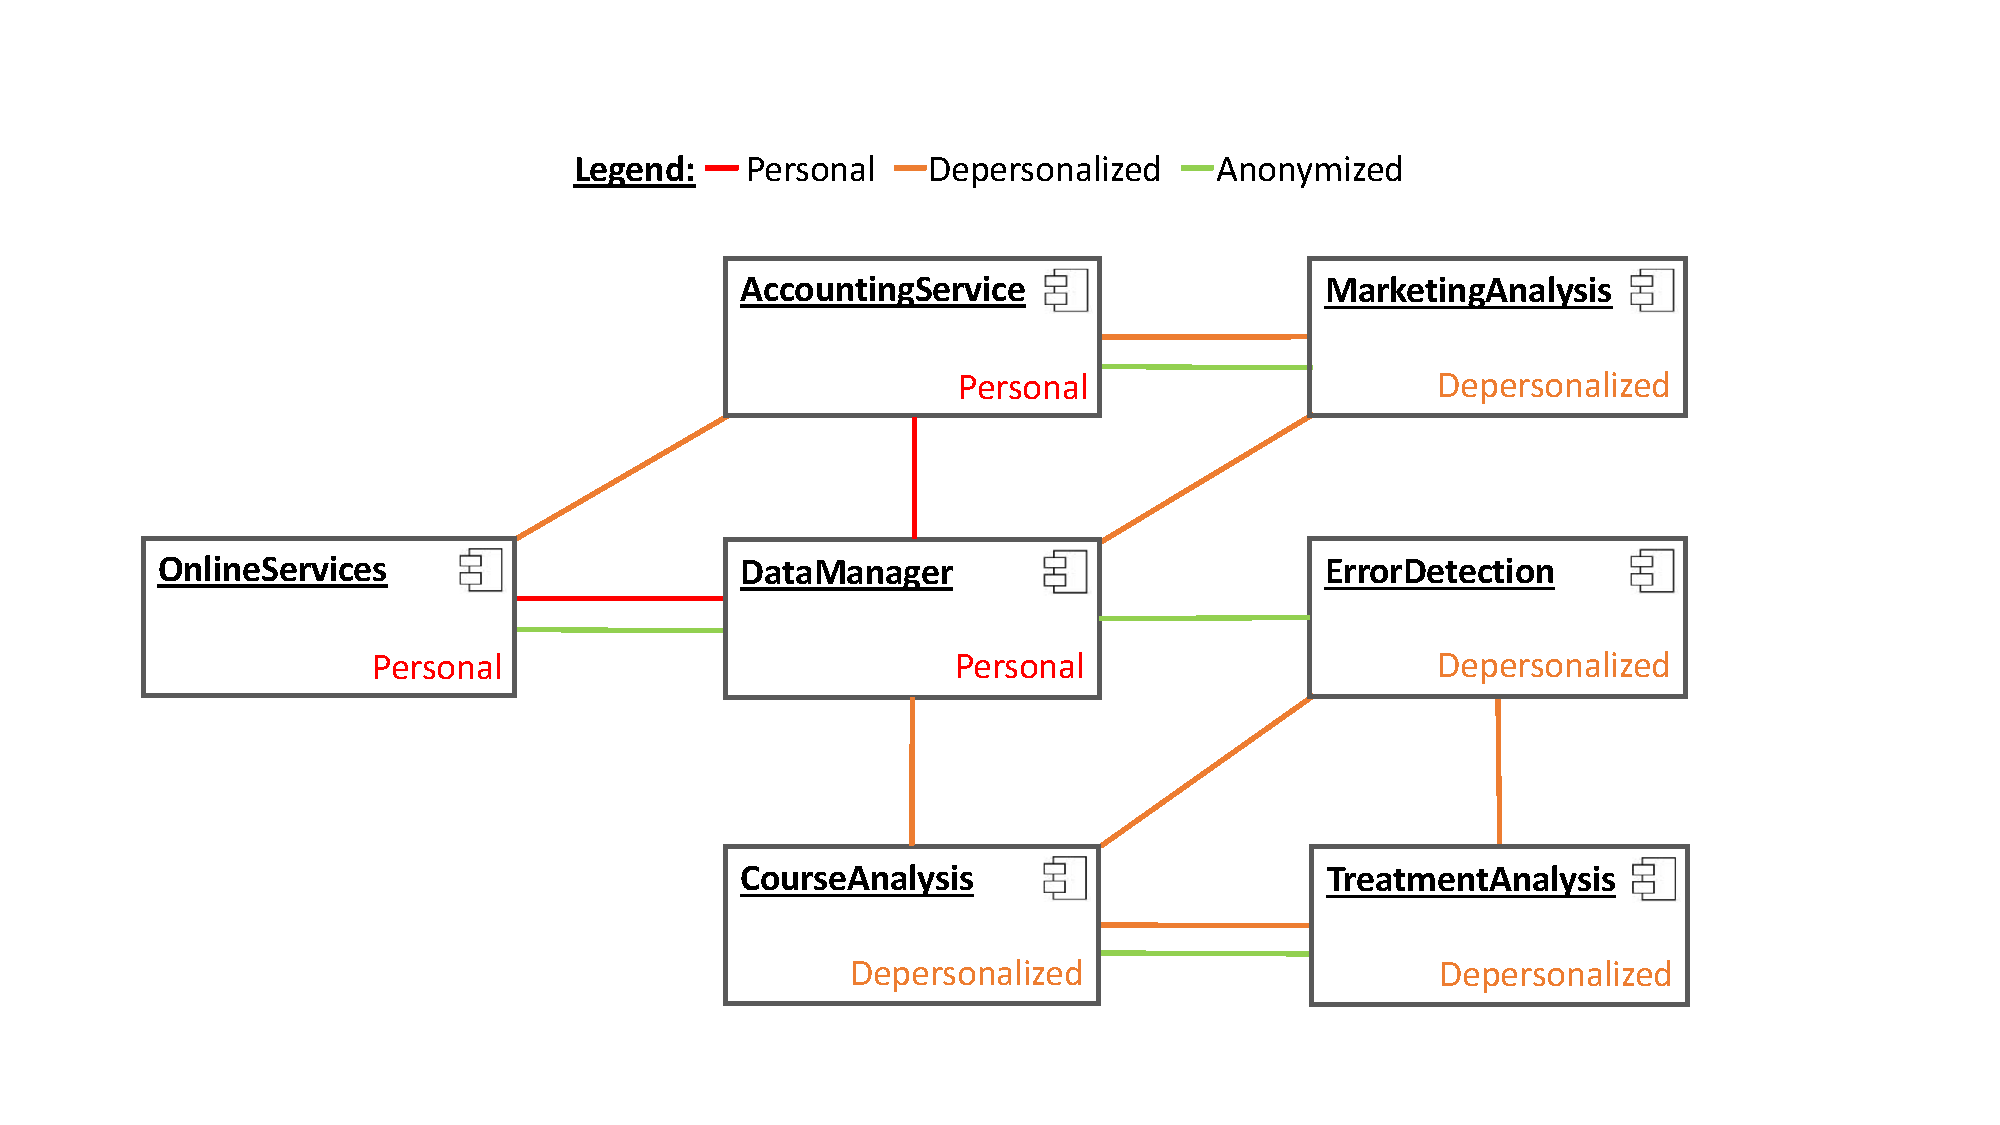
\includegraphics[trim = 20mm 10mm 40mm 10mm, clip, width=0.99\textwidth]{graphs/medSys_eval_pa_tagging_init}
		\caption{Initial categorization}
		\label{fig:eval:pa:base_tag}
	\end{minipage}
	\begin{minipage}[b]{0.48\textwidth}
		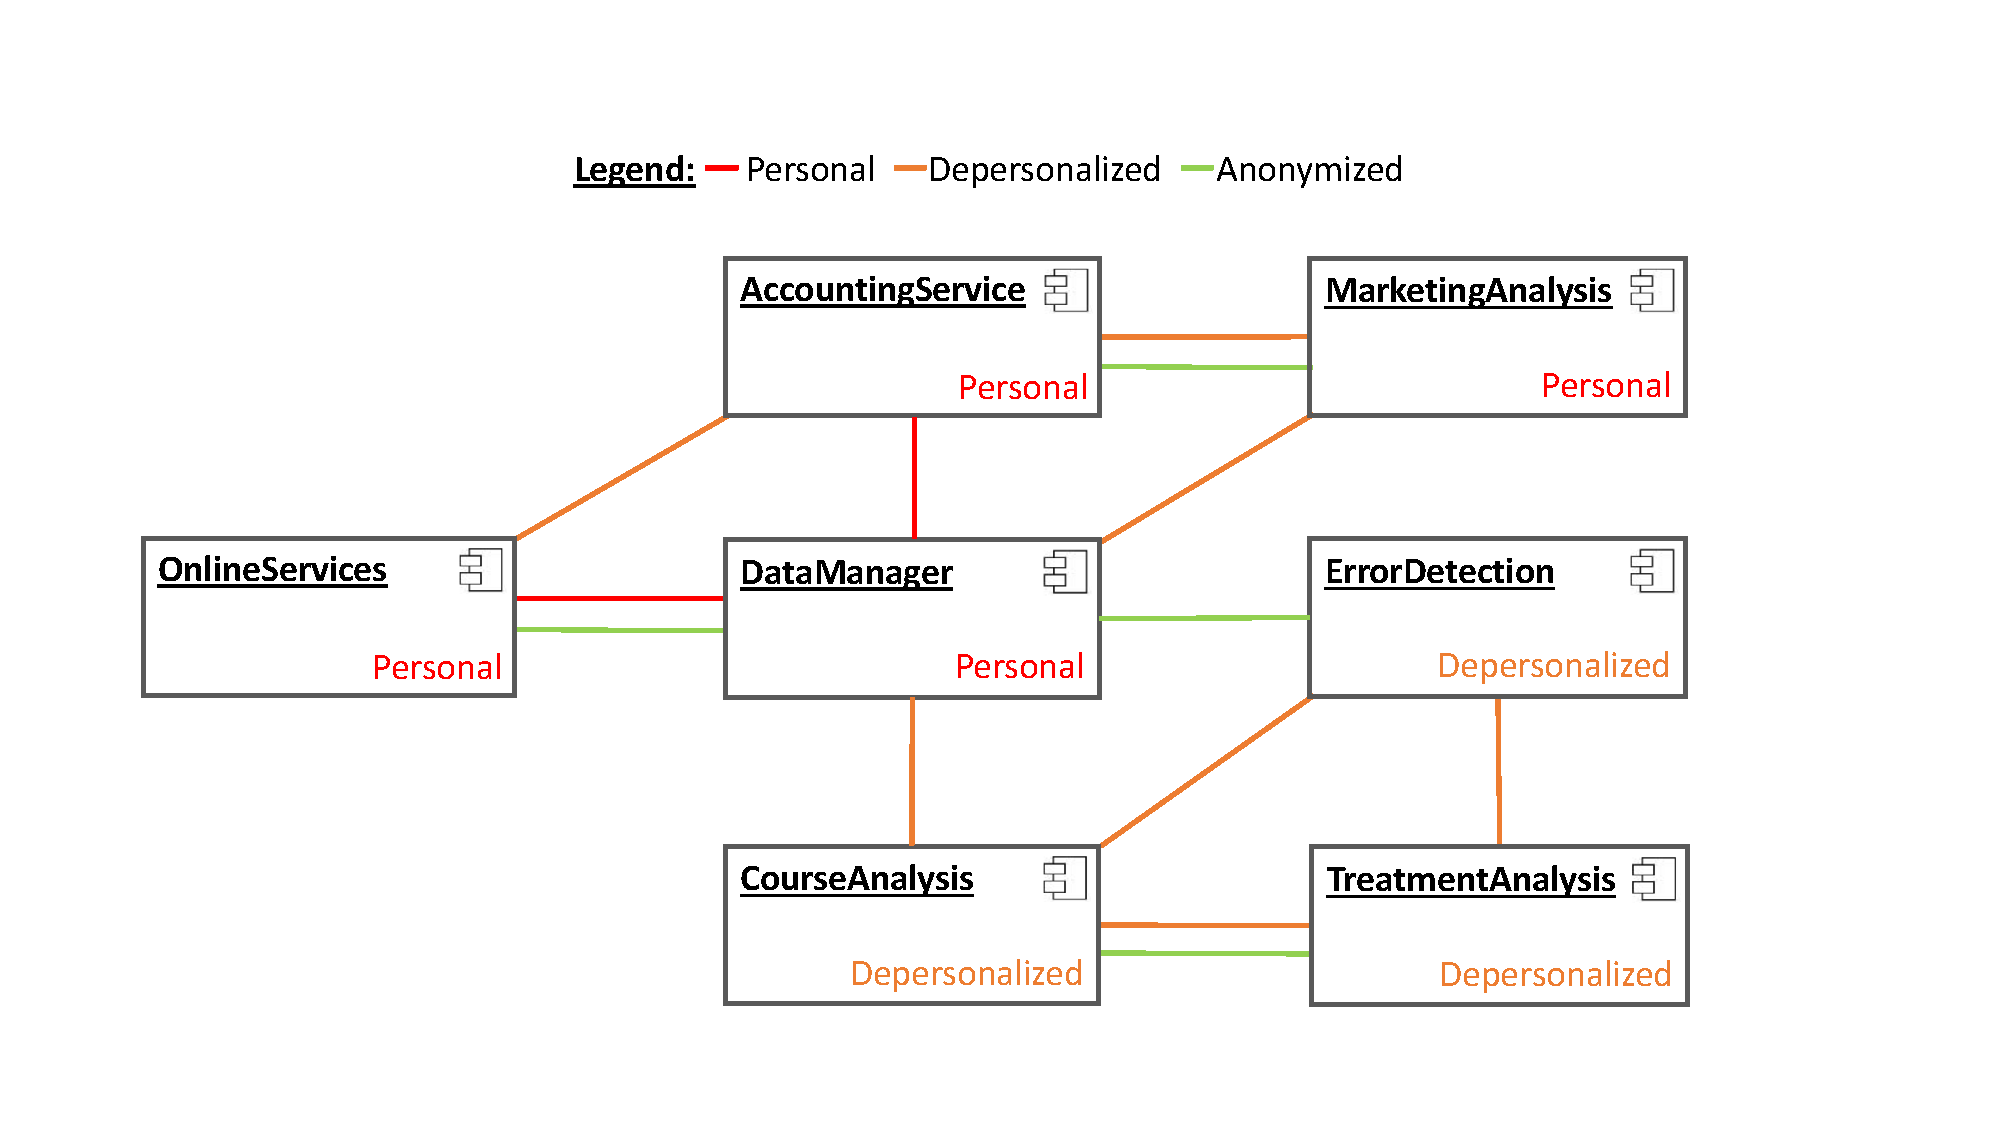
\includegraphics[trim = 20mm 10mm 40mm 10mm, clip, width=0.99\textwidth]{graphs/medSys_eval_pa_tagging_analysis}
		\caption{Categorization analysis result}
		\label{fig:eval:pa:categorized}
	\end{minipage}
\end{figure}

After the execution we calculated a \textit{Jaccard Coefficient} of \textit{1.0}. This shows us that the pipeline trigger was correctly processed. \autoref{fig:eval:pa:base_tag} shows the initial component categorization, \autoref{fig:eval:pa:categorized} shows the categorization analysis result. This states show, that our expectations on the component categorization, $C1, C2$ and $C3$, were met. The deployment analysis reports a legal deployment, which is also what we anticipated. So, the results are true to our expectations.

To trigger the pipeline another time, we will deploy the \textit{GovStatistics} component onto \textit{Server2}. The component must be tagged depersonalised and the deployment analysis must report a \textit{joining data stream} on \textit{Server2} $(D2)$.

\begin{figure}[h]
	\centering
	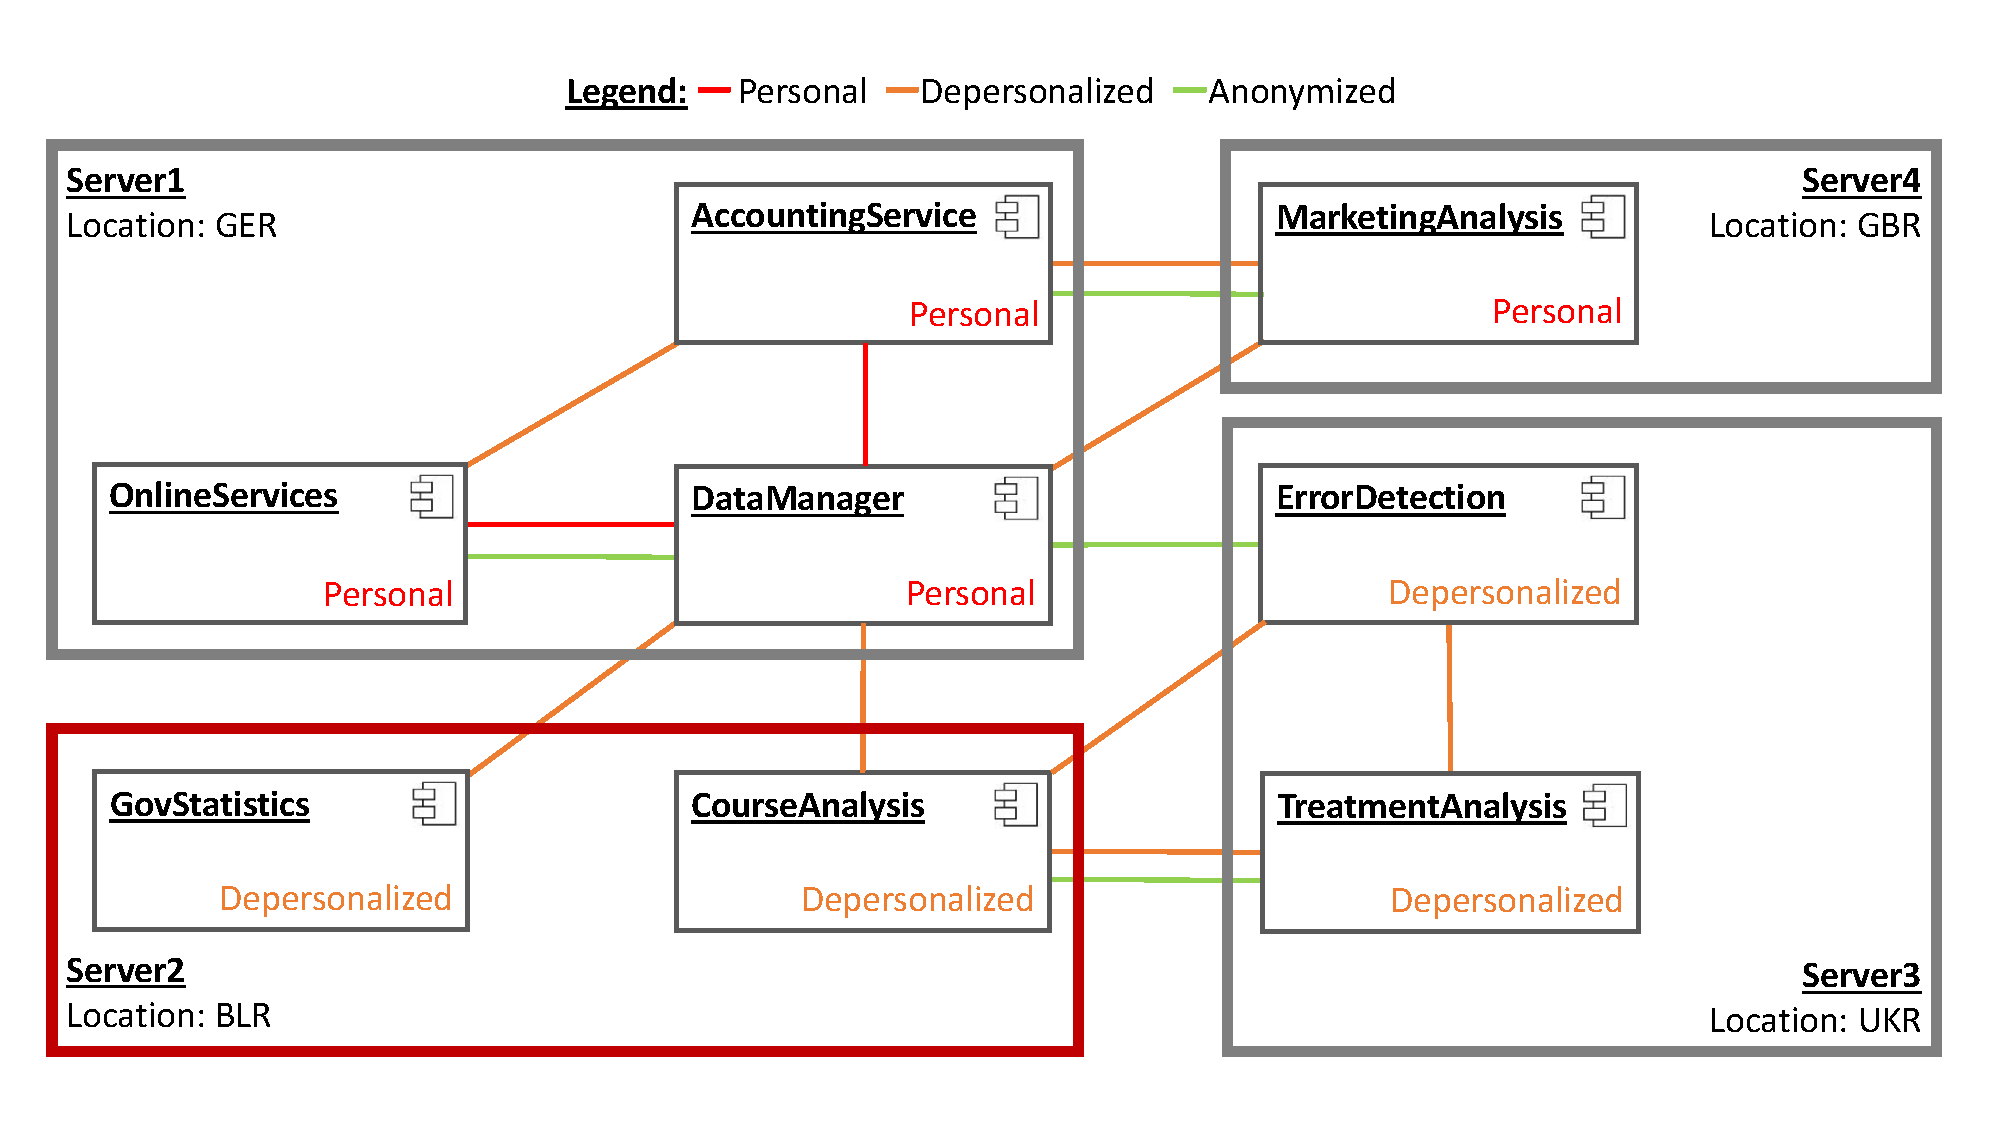
\includegraphics[trim = 0mm 10mm 0mm 10mm, clip, width=0.90\textwidth]{graphs/medSys_eval_pa_da}
	\caption{Deployment analysis result (1)}
	\label{fig:eval:pa:depl_ana}
\end{figure}

\autoref{fig:eval:pa:depl_ana} visualises the component categorization and deployment analysis result. The execution of the second pipeline trigger, reports a privacy violation. The cause is a joining data stream on Server2. This is what we provoked and expected $(D2)$. The \textit{Jaccard Coefficient} for the trigger processing is \textit{1.0}, again.

For the final pipeline trigger, we will migrate \textit{Server2} into the EU, to Italy. We expect, that the server no longer reports a illegal deployment, despite the potential \textit{joining data stream} on the server $(D3)$. During the migration, \textit{Great Britain} is removed from the \textit{save} country list, due to a management decision. As a consequence, we predict a new privacy violation concerning the deployment of the personal \textit{MarketingAnalysis} component on \textit{Server4} $(D1)$.

\begin{figure}[h]
	\centering
	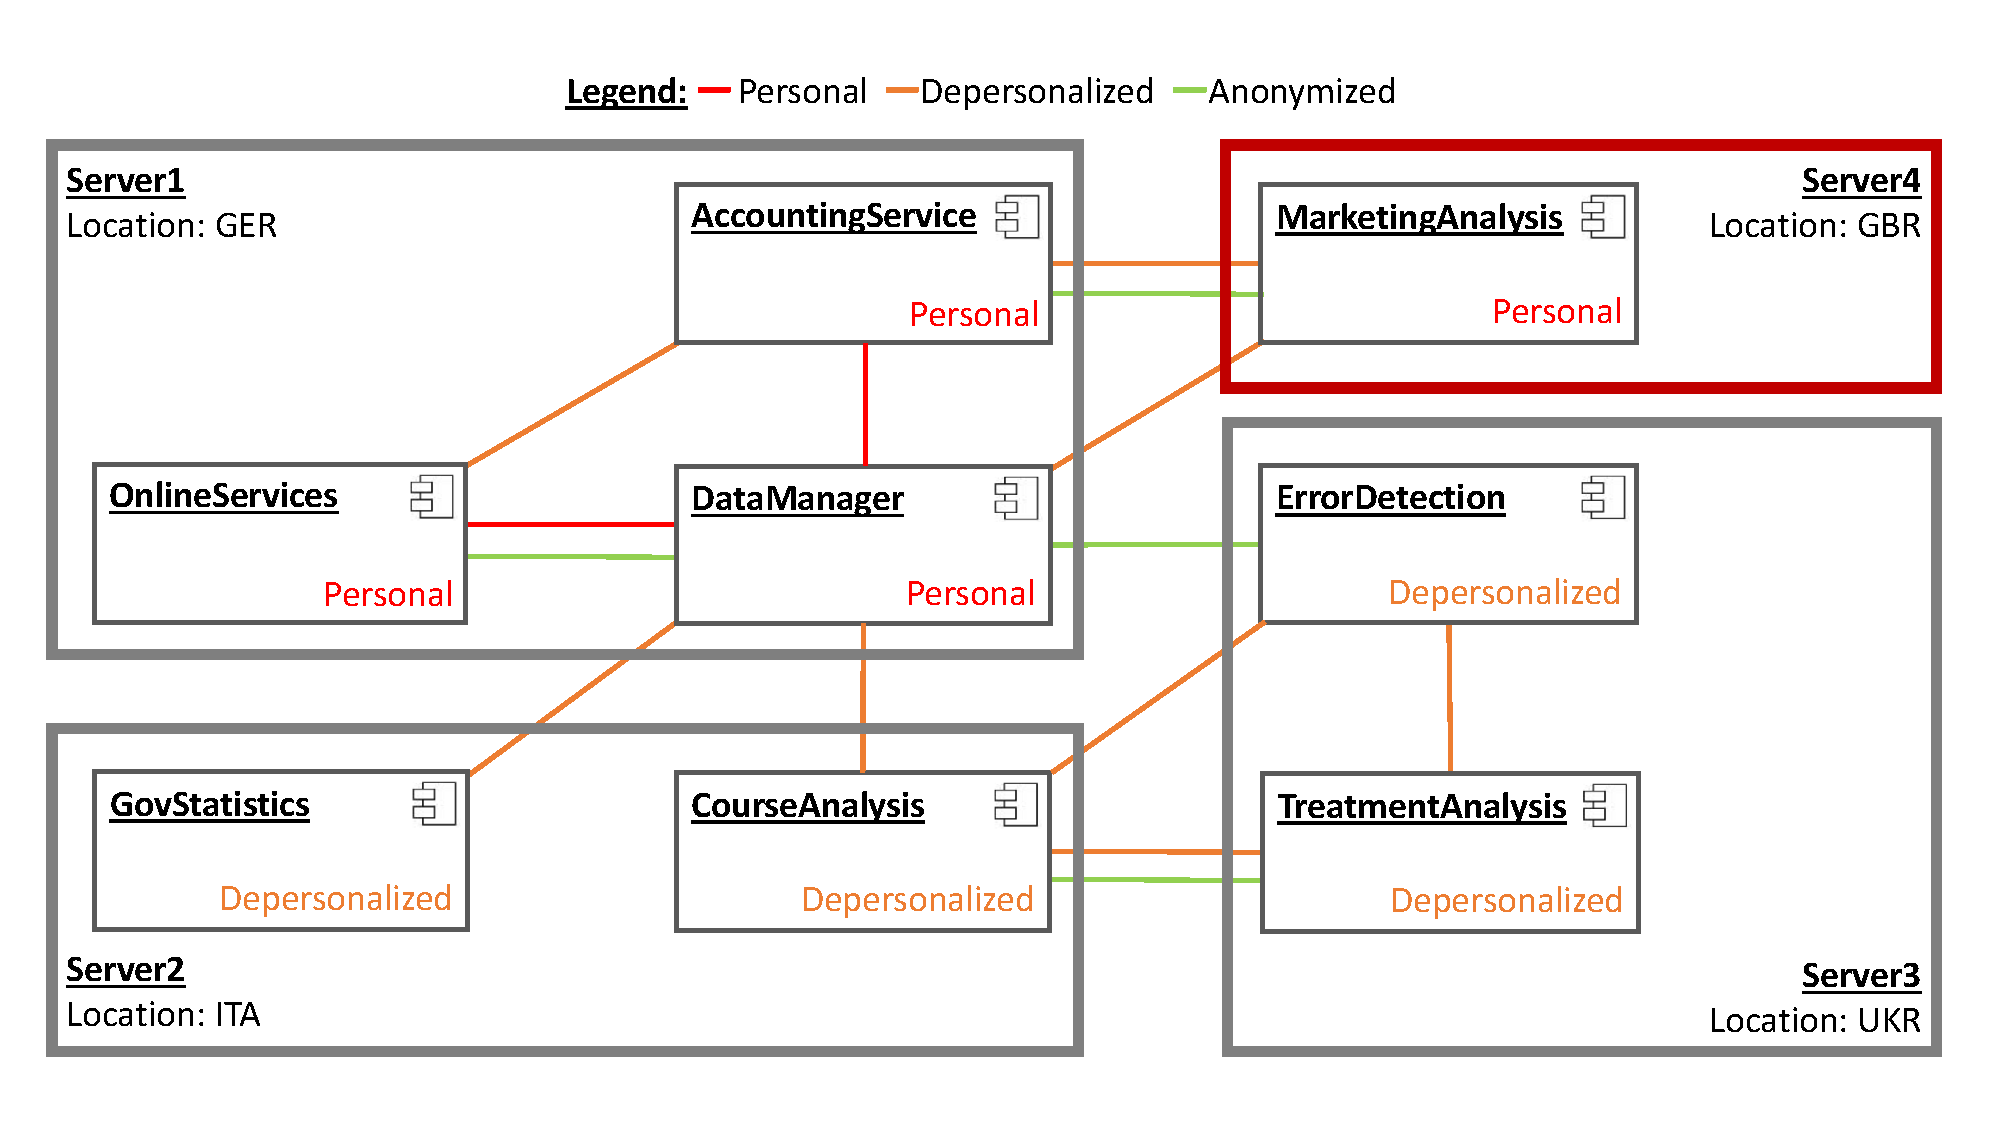
\includegraphics[trim = 0mm 10mm 0mm 10mm, clip, width=0.90\textwidth]{graphs/medSys_eval_pa_da_2}
	\caption{Deployment analysis result (2)}
	\label{fig:eval:pa:depl_ana_2}
\end{figure}

\autoref{fig:eval:pa:depl_ana_2} shows the final trigger result. As expected, the \textit{Marketing Analysis} deployment on \textit{Server4} is reported as privacy violation. Further, \textit{Server2} is now privacy compliant. The \textit{Jaccard Coefficient} is \textit{1.0}, so the geo-location transformation was successfully executed. The result is true to our expectations, this means, we have successfully shown $D1$ and $D3$.

We have shown, that the \textit{Component Classification} algorithm and the \textit{Deployment Analysis} works as intended. Further, we proofed the concept of a privacy analysis on an architectural level as intended in \autoref{sec:Introduction:goals} (\textbf{RQ-A1}). We exemplary showed the correctness of the component categorization and the deployment analysis. This includes the two major tasks of detecting joining data streams on component categorization and deployment analysis level. Further, we showed the correct identification of a set of components, located on a server, sharing a single depersonalised component as a data source. So, concerning \textbf{RQ-A2}, we have a perfect accuracy. Further, exemplary privacy violations will be used in the other accuracy evaluations.

\subsection{Privacy Analysis: Scalability Evaluation}
\label{sec:Evaluation:privacyanalysis:scale}

For the scalability evaluation of the privacy analysis, we will use the generated model (\autoref{sec:Evaluation:models:generated}), since models of the intended scale are not constructable by hand.

The time measurement starts before the graph is constructed from the model. Time measures are taken for the component classification and the deployment analysis. Complex console outputs, like the system structure, are deactivated to minimise random performance influences.

We measure a graph size of 10 to one million nodes on a logarithmic scale. The model set-up was described in \autoref{sec:Evaluation:models:generated}. The \textit{legal} geo-locations consist of 40 random chosen countries, while the server geo-locations are distributed among roughly 200 countries. This proportion was chosen to provoke many privacy violations and a significant amount of \textit{joining data stream} analysis. Each model measurement is repeated ten times to minimize runtime effects.

\begin{figure}[h]
	\centering
	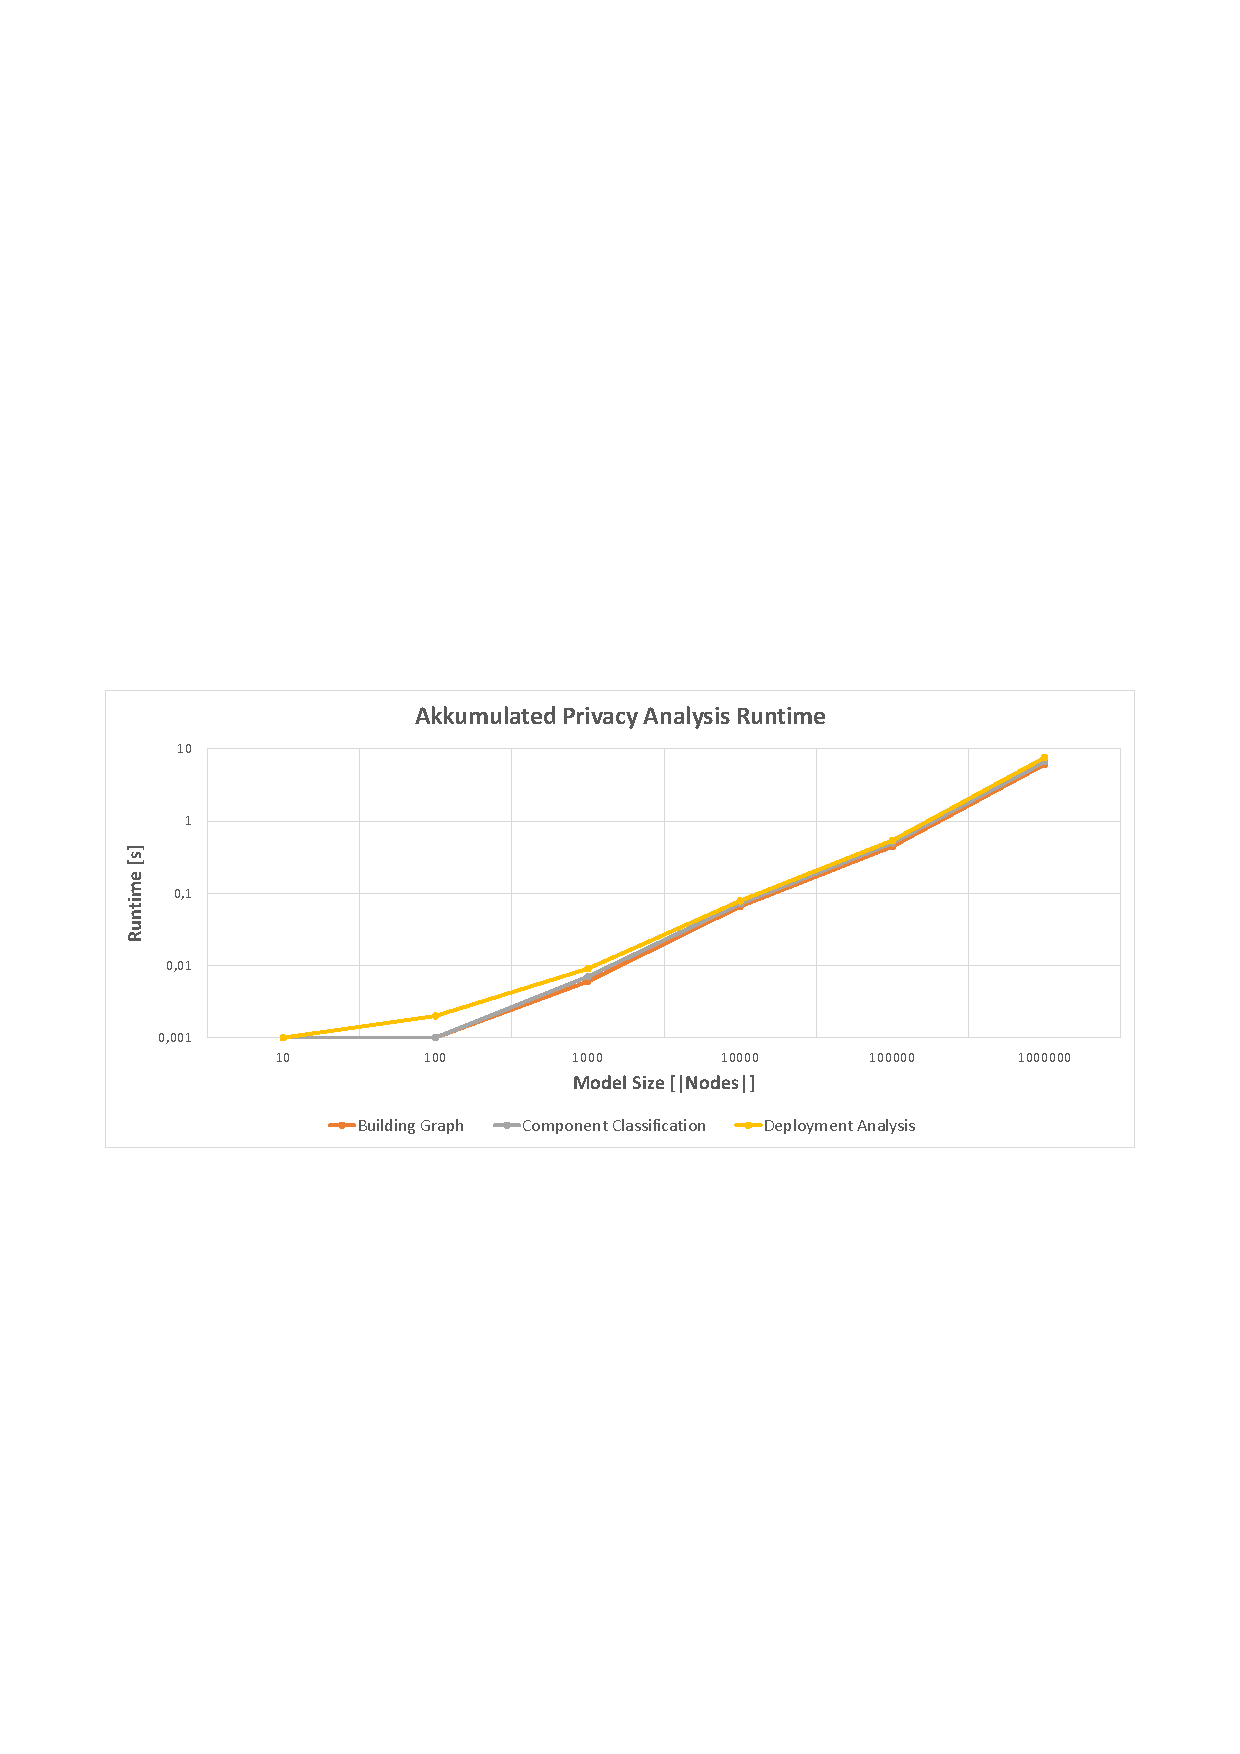
\includegraphics[trim = 15mm 95mm 13mm 110mm, clip, width=0.95\textwidth]{graphs/Runtime_pa}
	\caption{Privacy Analysis runtime}
	\label{fig:eval:pa:runtime}
\end{figure}


\begin{figure}[h]
	\centering
	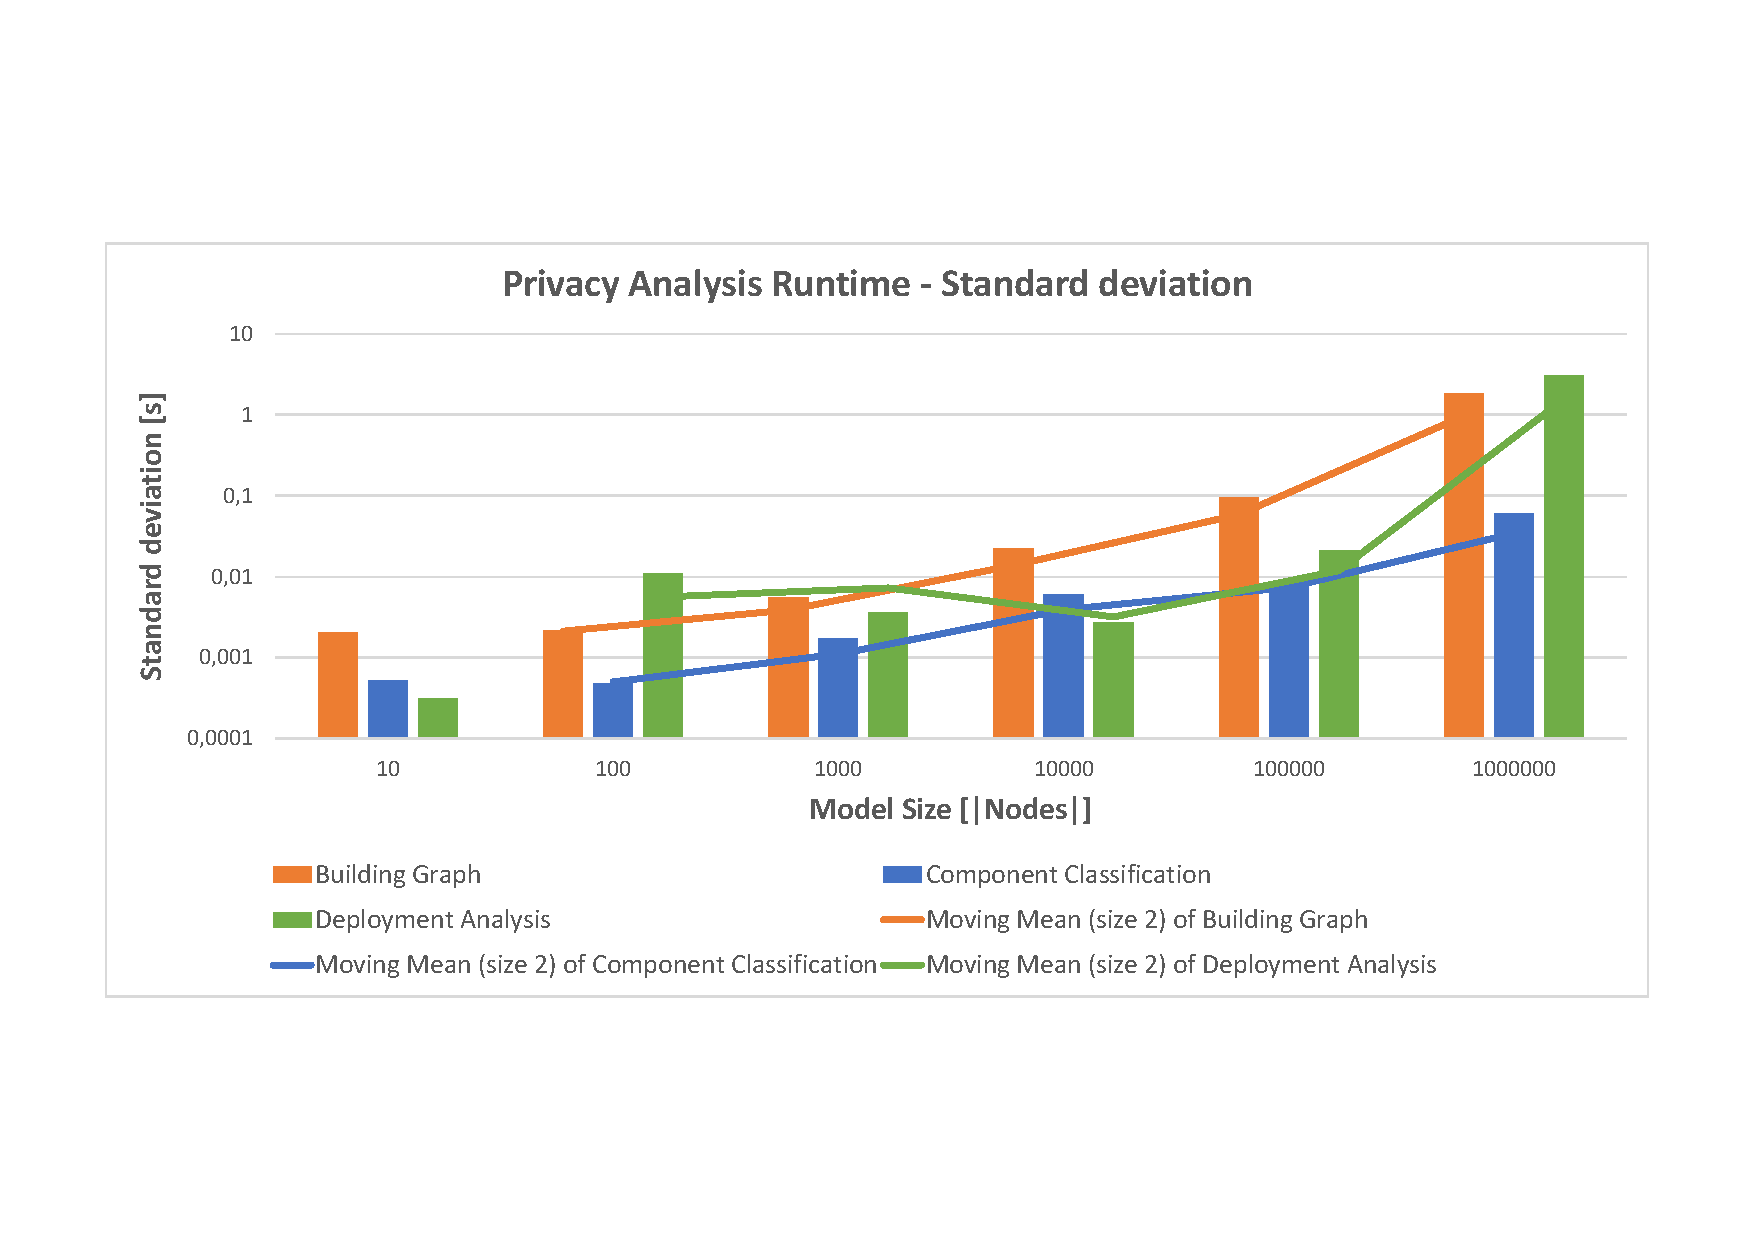
\includegraphics[trim = 5mm 30mm 10mm 30mm, clip, width=0.95\textwidth]{graphs/Runtime_pa_sd}
	\caption{Privacy Analysis runtime standard deviation}
	\label{fig:eval:pa:runtime_sd}
\end{figure}

\autoref{fig:eval:pa:runtime} shows the accumulated runtime in the order the tasks are executed. Initially, the graph for the privacy analysis is created, followed by the component classification and finally the deployment analysis. The graph shows a nearly linear increasing runtime. The major time is consumed by the graph construction, while the component classification and deployment analysis only show minor size effects. The accumulated runtime for one million nodes is still significantly below ten seconds. The limiting task for further scalability tests is the graph generation due to memory limitations and java \textit{HashMap} overflow errors. However, graphs with the size of 1000 and more nodes are already very unlikely.

The standard deviation \autoref{fig:eval:pa:runtime_sd} is increasing - in general - linear with the model size. The deployment analysis however, shows some irregular behaviour. This could be due to the randomly selected save countries. A standard deviation of three times the actual mean runtime shows significantly runtime computation differences. Nevertheless, a maximum deployment analysis time of ten seconds on a one million nodes graph is still considered very fast. And an overall privacy analysis runtime of maximum 15 seconds is also very quick. So, concerning the research question \textbf{RQ-A3}, we can argue, that the privacy analysis has good scaling characteristics and a very fast execution time.


\section{Model Generation}
\label{sec:Evaluation:generation}

The privacy compliant model generation is only evaluated under the \textit{Accuracy} aspect. The \textit{Scalability} evaluation was already performed by the creators of PerOpteryx (see \cite{Koziolek.2014}) and our Privacy Analysis was evaluated in \autoref{sec:Evaluation:privacyanalysis}. We will focus on the problem specified in \autoref{sec:Introduction:problems}, the generation of a privacy compliant re-deployment model.

For this evaluation we use the CoCoME model (\autoref{sec:eval:models:cocome}) together with the scenarios \#2 (\autoref{eval:scenario:2}) and \#4 (\autoref{eval:scenario:4}). Scenario \#2 describes a complete iObserve Privacy execution, including the successful execution of PerOpteryx for the re-deployment model generation. Scenario \#4 describes the case, in which PerOpteryx fails to generate a privacy compliant candidate. We will start with Scenario \#2.

We deploy the CoCoME components on one EU server each and adjust the individual server costs to reflect EU and Non-EU status (see \autoref{ch:PerOpt}). We will trigger the pipeline by moving the \textit{Server4-EU}, which hosts the component, categorised as personal, \textit{webservice.inventory}, to Ukraine.

After the execution of our model generation framework, \textit{PerOpteryx}, we expect the re-deployment model to be privacy compliant. This is the major concern and primary focus. However, we further anticipate a deployment with fewer server in use, as well as a migration of multiple \textit{depersonalised} components to Non-EU servers.

PerOpteryx is configured to execute \textit{four iterations} with \textit{20 candidates} per iteration. This means, a total of 80 candidates will be created and evaluated. 


\begin{table}[h]
	\centering
	\begin{tabular}{ r | l | l | l }
		\hline
		\textbf{Component} & \textbf{Categorization} & \textbf{Deployment} & \textbf{Redeployment} \\
		\hline
		cloud.web & Depersonalized & Server1-EU & Server6-EU \\
		tradingsystem.inventory & Personal & Server2-EU & Server1-EU \\
		cashdeskline.cashdeskservice & Depersonalized & Server3-EU & Server2-NonEU \\
		webservice.inventory & Personal & Server4-EU & Server6-EU \\
		tradingsystem.cashdeskline & Depersonalized & Server5-EU & Server4-EU \\
		tradingsystem.external.Bank & Depersonalized & Server6-EU & Server3-NonEU \\
		\hline
	\end{tabular}
	\caption{Component categorization, runtime deployment and re-deployment}
	\label{tab:eval:gen:execution}
\end{table}

The \autoref{tab:eval:gen:execution} shows the components, their data privacy level classification, the initial deployment and the generated re-deployment. A performed privacy analysis on the re-deployment model shows, that the model is privacy compliant. So, the major goal (see \autoref{sec:Introduction:goals}) was accomplished. Further, depersonalised components were moved to more cheap Non-EU severs and two components were deployed onto the same server. Both deployment goals indicate, that the \textit{most cost efficient} model was chosen - as intended. However, no component stays at this original server, which produces (unnecessary) migration costs. The execution time of PerOpteryx was about 30 seconds and elven of 80 candidates were privacy compliant.

In scenario \#4, no privacy compliant re-deployment model can be found, PerOpteryx crashes or any kind of error occurs. However, the end result stays unchanged, no valid re-deployment model is available after the PerOpteryx execution. We are provoking this situation by deploying all components onto a single server. As the pipeline trigger we are moving this server to a Non-EU geo-location. We expect iObserve Privacy to report, that no privacy compliant PCM model was found. Basically, we expect, that iObserve invokes the \textit{operator-in-the-loop} for manual error treatment.

The execution shows an error, which states, that the given re-deployment model is not privacy compliant. If a listener would be registered, the listener would have been notified. The execution lives up to our expectations.

Concerning the research questions in \autoref{sec:Introduction:goals}, we have shown that we are able to generate a privacy compliant re-deployment model (\textbf{RQ-P1}) and that we are able to invoke the \textit{operator-in-the-loop} on an error situation (\textbf{RQ-P2}).

\section{System Adaptation}
\label{sec:Evaluation:planning}

The Adaptation Planing, described in \autoref{ch:SysAdap}, aims for calculating a sequence of adaptation actions. The execution of this adaptation order must result in a runtime model, that is equivalent to the redeployment model. This is one of the research goals stated in \autoref{sec:Introduction:goals}. We will evaluate this task towards its accuracy and scalability.

 
\subsection{Adaptation: Accuracy Evaluation}

We will continue with scenario \#2 from the generation evaluation (\autoref{sec:Evaluation:generation}). This means, we use the input model from model generation, as well as the calculated re-deployment model to calculate the adaptation sequence. We will show the correctness of the adaptation sequence calculation, by translating the adaptation order to an equivalent iObserve privacy input event sequence. After \textit{iObserve privacy} processed the events, the \textit{Jaccard Coefficient} - between the computed re-deployment model from PerOpteryx and the iObserve runtime model - must be \textit{1.0}. As mentioned, this example shows the continues MAPE loop and is therefore as close as possible to a real world example.

%re-establishing the privacy compliance. to show the MAPE loop validity. To show, that the given adaptation order leads to a privacy compliant system, we will simulate the adaptation. This will be achieved by 

We expect the calculated adaptation sequence to represent a series of adaptation actions that migrates the runtime model towards the re-deployment model. Further, we anticipate the order to be sorted after the \textit{Unversal Action Order} specified in \autoref{tab:SysAdap:order}.
This means, the sequence is initially \textit{acquiring} the newly used servers, followed by a series of \textit{migration} actions, that move the components to their new servers. Finally there should be three \textit{terminate} actions to release the servers, that are no longer needed. 

\begin{table}[h]
	\centering
	\begin{tabular}{r | l  l l l}
		\hline
		\textbf{Action} & \multicolumn{3}{ l }{\textbf{Values}}\\
		\hline
		Acquire & \multicolumn{3}{ l }{Server3-NonEU} \\
		Acquire & \multicolumn{3}{ l }{Server2-NonEU} \\
		Migrate & webservice.inventory & Server4-EU & -> & Server6-EU \\
		Migrate & tradingsystem.cashdeskline & Server5-EU & -> & Server4-EU \\
		Migrate & tradingsystem.external.Bank & Server6-EU & -> & Server3-NonEU \\
		Migrate & cashdeskline.cashdeskservice & Server3-EU & -> & Server2-NonEU \\
		Migrate & cloud.web & Server1-EU & -> & Server6-EU \\
		Migrate & tradingsystem.inventory & Server2-EU & -> & Server1-EU \\
		Terminate & \multicolumn{3}{ l }{Server3-EU} \\
		Terminate & \multicolumn{3}{ l }{Server2-EU} \\
		Terminate & \multicolumn{3}{ l }{Server5-EU} \\
		\hline
	\end{tabular}
	\caption{The ordered adaptation sequence}
	\label{tab:eval:adapt:action_order}
\end{table}

\autoref{tab:eval:adapt:action_order} shows the output adaptation sequence for scenario \#2. The result is true to our expectations. The \textit{Unversal Action Order} is met. For the transformation onto iObserve input events, we can ignore the acquire actions, since the resource containers already exist in the resource environment model. Every migrate action needs to be translated into two events: a \textit{Undeployment} event and a \textit{Deployment} event. The terminate actions can also be ignored, since there is no real server to release or terminate. We expect the system to be in a privacy compliant state after the execution of the iObserve input events. \autoref{tab:eval:adapt:action_input_result} shows the resulting iObserve input events.

\begin{table}[h]
	\centering
	\begin{tabular}{r | l}
		\hline
		\textbf{Action} & \textbf{Values}\\
		\hline
		UnDeployment & webservice.inventory from Server4-EU\\
		Deployment & webservice.inventory on Server6-EU\\
		
		UnDeployment & tradingsystem.cashdeskline from Server5-EU\\
		Deployment & tradingsystem.cashdeskline on Server4-EU\\
		
		UnDeployment & tradingsystem.external.Bank from Server6-EU\\
		Deployment & tradingsystem.external.Bank on Server3-NonEU\\
		
		UnDeployment & cashdeskline.cashdeskservice from Server3-EU\\
		Deployment & cashdeskline.cashdeskservice on Server2-NonEU\\
		
		UnDeployment & cloud.web from Server1-EU\\
		Deployment & cloud.web on Server3-EU\\
		
		UnDeployment & tradingsystem.inventory from Server2-EU\\
		Deployment & tradingsystem.inventory on Server1-EU\\
		\hline
	\end{tabular}
	\caption{iObserve input event translated adaptation sequence}
	\label{tab:eval:adapt:action_input_result}
\end{table}


The execution of the transformed adaptation sequence (\autoref{tab:eval:adapt:action_input_result}) results in a privacy compliant PCM model and the \textit{Jaccard Coefficient} of the post-execution runtime model and the calculated redeployment model is \textit{1.0}. So, the result fulfills our expectations and solves the in \autoref{sec:Introduction:problems} stated research question \textbf{RQ-E1} concerning \textit{automated privacy compliance re-establishment}.

\begin{figure}[h]
	\centering
	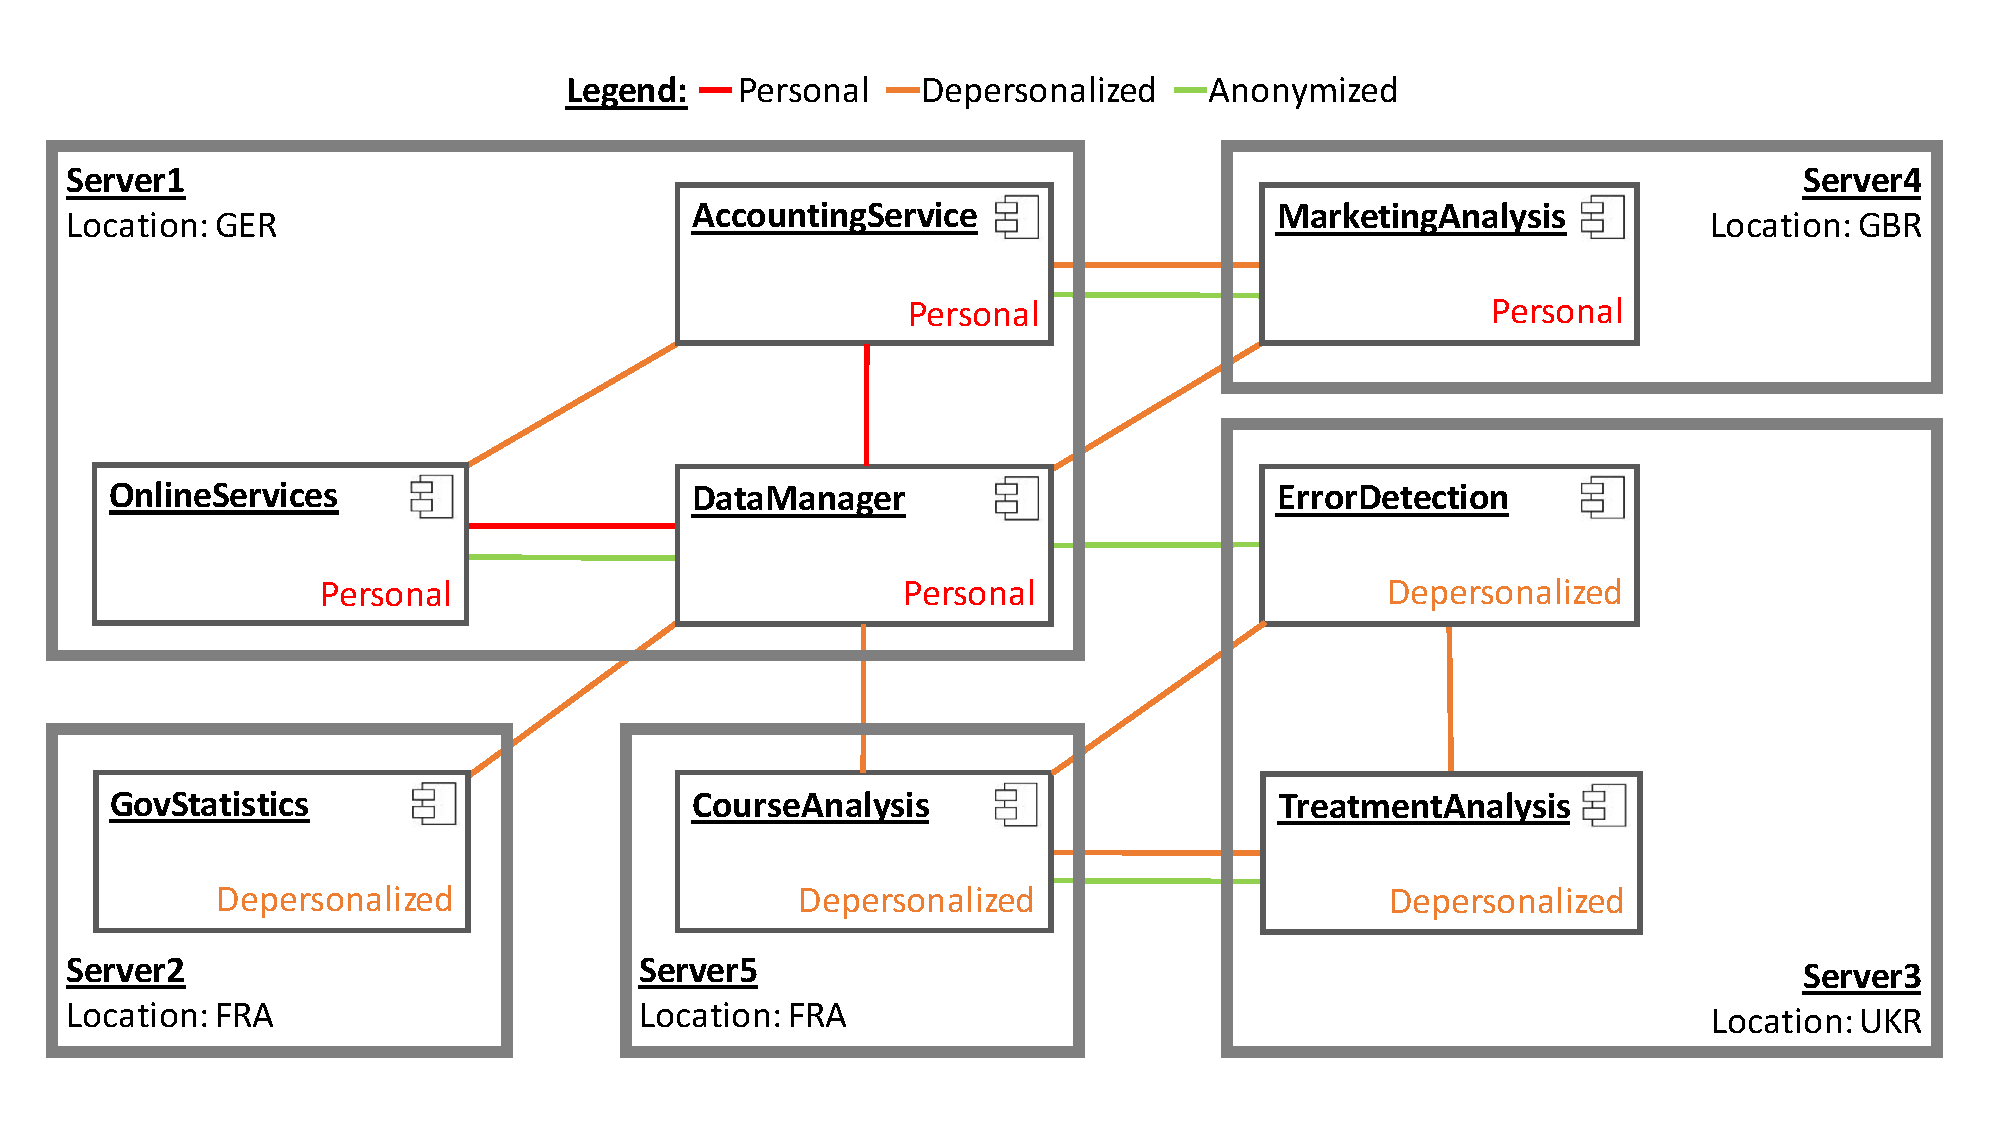
\includegraphics[trim = 5mm 10mm 10mm 10mm, clip, width=0.65\textwidth]{graphs/medSystem_adap_calc_all_runtime}
	\caption{Runtime model}
	\label{fig:eval:adapt:4:run}
\end{figure}


We will continue to evaluate the \textit{System Adaptation} with scenario \#3 to show the limitations and so far unseen capabilities of the adaptation calculation. PerOpteryx only adapts the system given according to the \textit{Design Decision} model (see \autoref{ch:PerOpt}). For iObserve Privacy PerOpteryx will only produce acquire, migrate and terminate actions. These are (usually) automatically executable.

For this scenario the Medi-Sys is used. We will modify the Medi-Sys model to provoke one of each action. \autoref{fig:eval:adapt:4:run} shows the runtime model, \autoref{fig:eval:adapt:4:redepl} shows the re-deployment model. The anticipated difference between these models is shown in \autoref{tab:eval:adapt:4:action_provoke}. We expect each of the seven actions to be detected, except the \textit{replicate} action, since this is not (yet) supported by the adaptation calculation. It will be subsided by an \textit{aquire Server2-2} and an \textit{allocate GovStatistics on Server2-2}.

\begin{figure}[h]
	\centering
	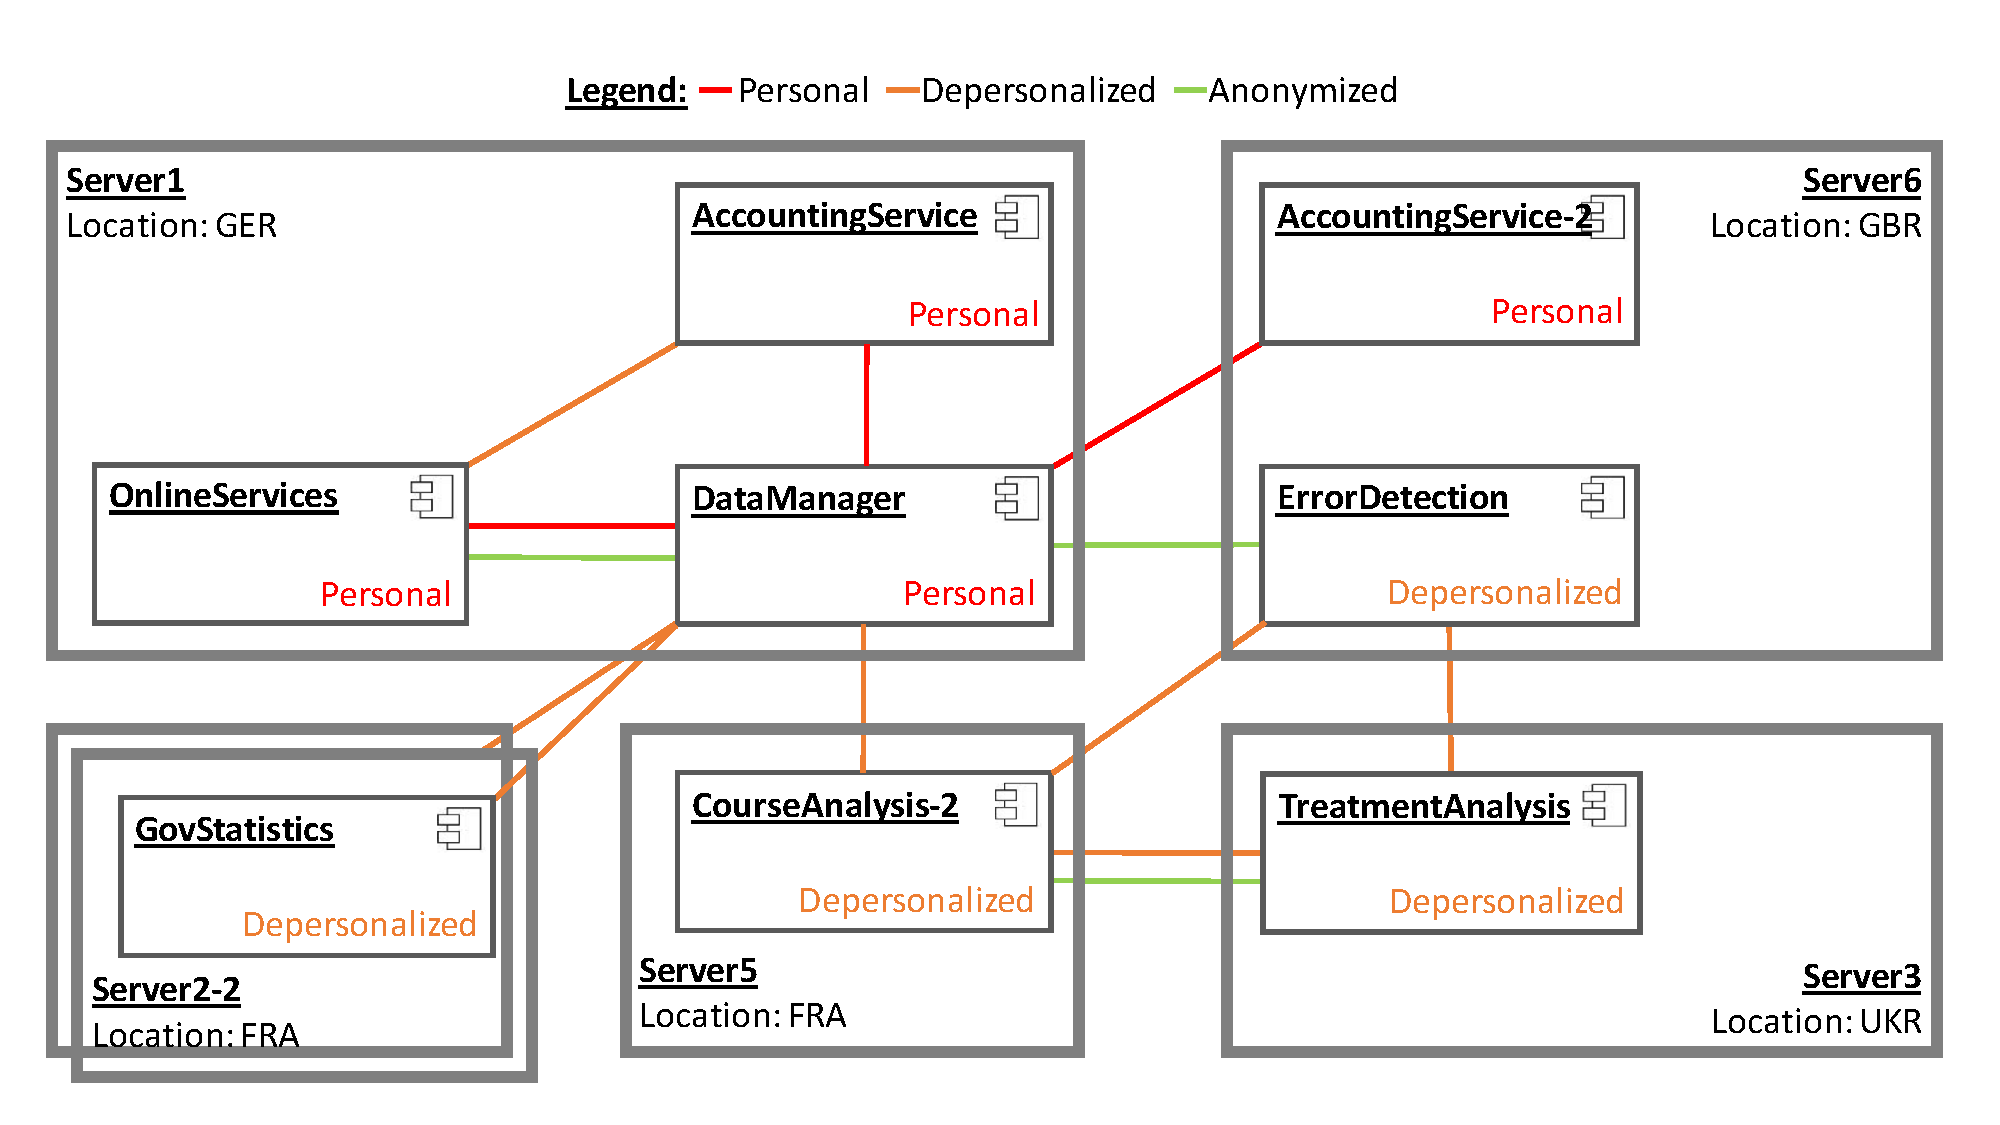
\includegraphics[trim = 5mm 5mm 10mm 10mm, clip, width=0.65\textwidth]{graphs/medSystem_adap_calc_all_redepl}
	\caption{Redeployment model}
	\label{fig:eval:adapt:4:redepl}
\end{figure}

\begin{table}[h]
	\centering
	\begin{tabular}{r | l }
		\hline
		\textbf{Action} & \textbf{Values}\\
		\hline
		Acquire & Server-6\\
		Exchange Component & CourseAnalysis to CourseAnalysis-2\\
		Deallocate & MarketingAnalysis from Server-4\\
		Allocate & AccountingService-2 on Server-6\\
		Migrate & ErrorDetection from Server-3 to Server-6\\
		Replicate & Server-2 (with GovStatistics)\\
		Terminate & Server-4\\
		\hline
	\end{tabular}
	\caption{Expected adaptation sequence for Scenario \#4}
	\label{tab:eval:adapt:4:action_provoke}
\end{table}

The execution of the adaptation calculation shows the expected result (see \autoref{tab:eval:adapt:4:action_result}). The replicate action is split into the expected \textit{acquire} and \textit{allocate} actions (marked with an *). To summarize, the results are true to our expectations.

\begin{table}[h]
	\centering
	\begin{tabular}{r | l }
		\hline
		\textbf{Action} & \textbf{Values}\\
		\hline
		Acquire & Server-6\\
		Acquire & Server2-2 (*)\\
		Exchange Component & CourseAnalysis to CourseAnalysis-2\\
		Allocate & AccountingService-2 on Server-6 (*)\\
		Allocate & GovStatistics-2 on Server2-2\\
		Deallocate & MarketingAnalysis from Server-4\\
		Migrate & ErrorDetection from Server-3 to Server-6\\
		Terminate & Server-4\\
		\hline
	\end{tabular}
	\caption{Expected adaptation sequence for Scenario \#4}
	\label{tab:eval:adapt:4:action_result}
\end{table}

Scenario \#4 intends to invoke the \textit{operator-in-the-loop}. We are unable to evaluate this scenario, since no technology dependent scripts (see \autoref{sec:SysAdap:exec}) for the actual execution are available to decide whether an action is automatically executable. This depends strongly on the used system binary management tools.

Concerning the research questions stated in \autoref{sec:Introduction:goals}, we have proved the concept of calculating an automated system adaptation sequence (\textbf{RQ-E1}). However, not all defined corner cases could be detected correctly. Nevertheless, the default real-world CoCoME example was successfully calculated and proven to be correct. Overall, \textbf{RQ-E2} shows a moderate to good accuracy.


\subsection{Adaptation: Scalability Evaluation}

For the scalability analysis we are using generated, logically valid PCM Privacy models (\autoref{sec:Evaluation:models:generated}). These models are randomly modified with respect to the logically validity. This means, that the model does not contain any errors like unconnected required interfaces, not allocated assembly contexts and deployments on non-existing resource containers. So, the model is error-free. We are measuring the time it takes to build the model graphs, as well as the time for the execution of the \textit{Adaptation Calculation} and the \textit{Adaptation Planning}.

The initial model is constructed as described in \autoref{sec:Evaluation:models:generated}. The modification is linear distributed over the acquire, terminate, allocate, deallocate, migrate and exchange component modifications. However, not every modification in the model leads to an adaptation action. The adding of another resource container is only recognized as an acquire action, if an assembly context is allocated on that new resource container. The termination of a resource container, that hosts one or more components, leads also to a migration action. With this in mind, we measure the time of the adaptation calculation and adaptation planning based on the amount of modifications in the model. The model itself is three times as big as the modifications provoked, so the anticipated amount of changes are possible. A model with 100 nodes can not contain 1000 modifications. We decided against a static model size due to long evaluation runs. Each measurement is repeated ten times, to reduce the impact of runtime effects. The input sizes are 10, 100, 1000 and 10000. An evaluation run with 100000 provoked changes was aborted after twelve hours of computation.

\begin{figure}[h]
	\centering
	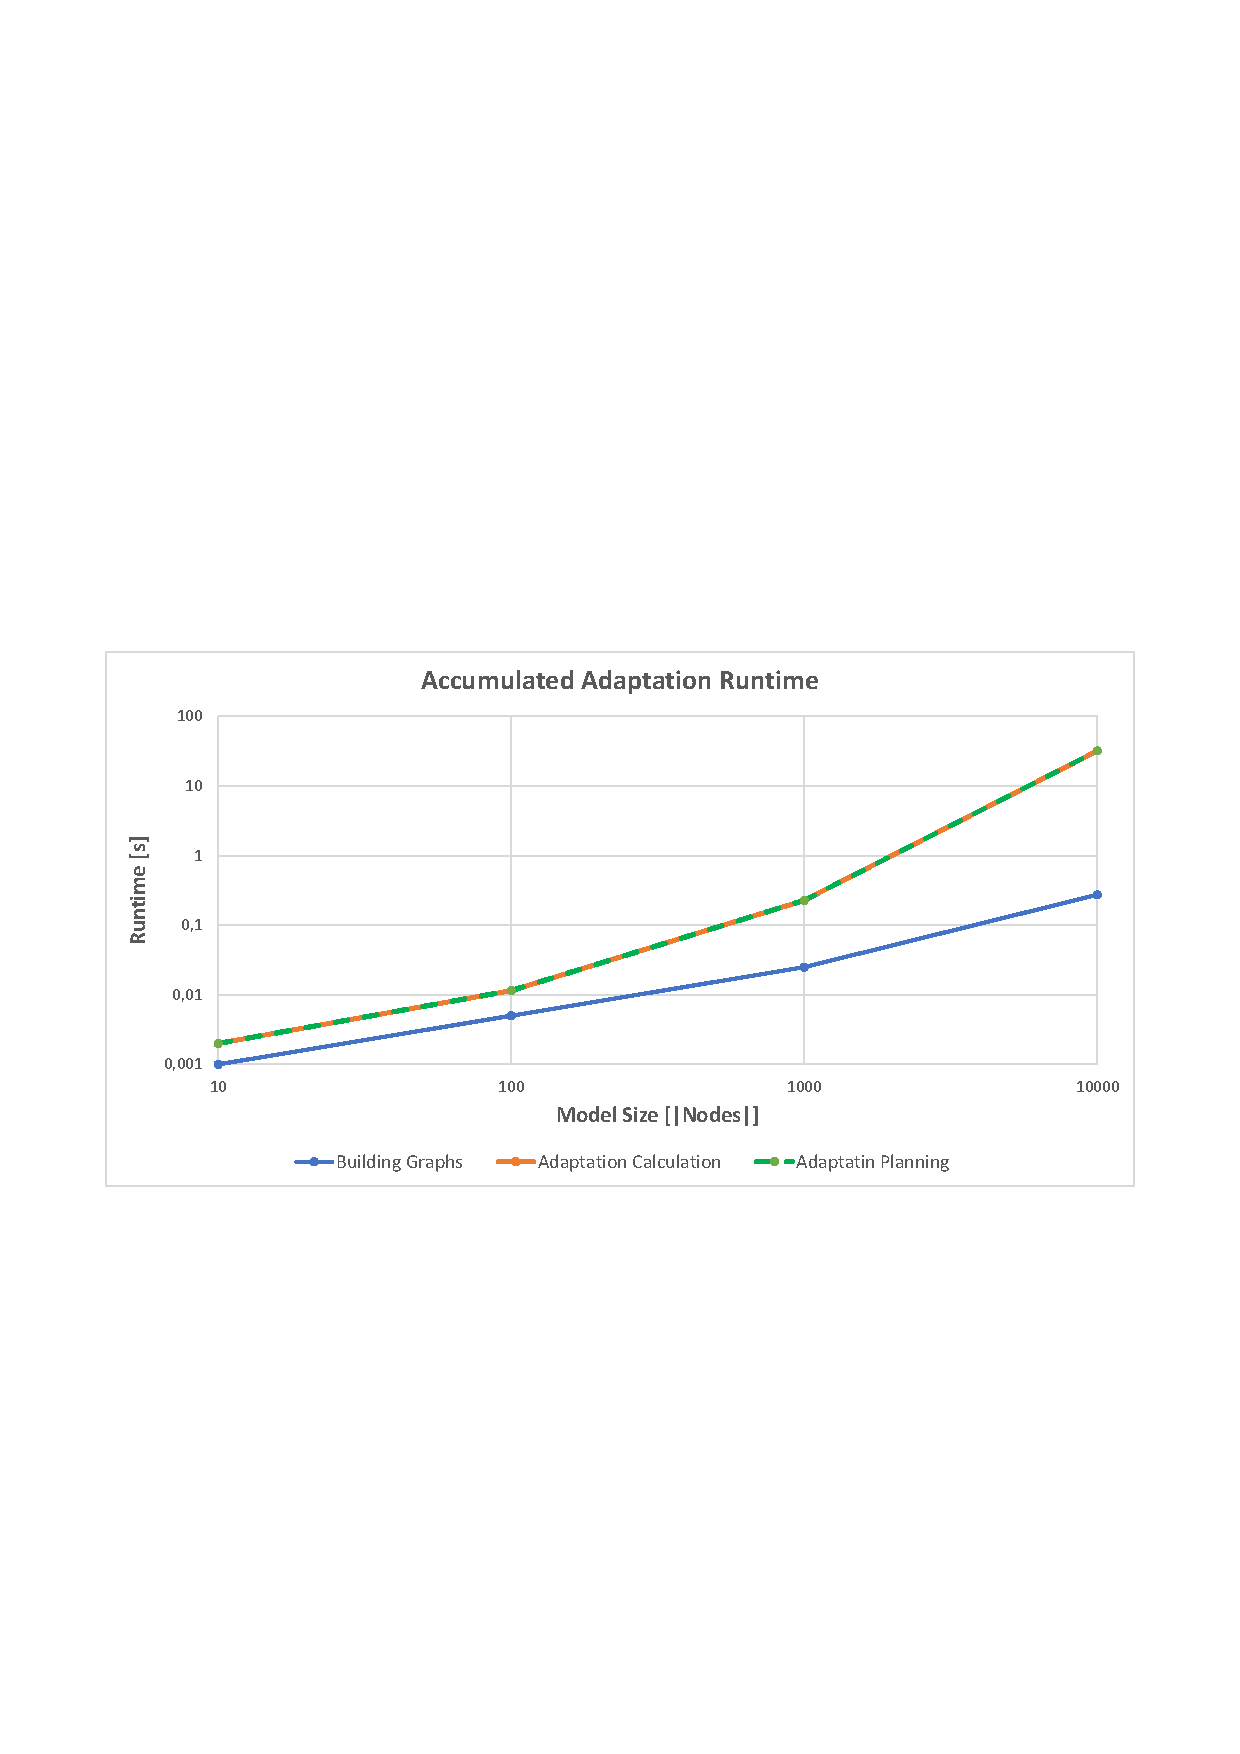
\includegraphics[trim = 15mm 95mm 15mm 105mm, clip, width=0.90\textwidth]{graphs/Runtime_adapt}
	\caption{Adaptation runtime}
	\label{fig:eval:adap:runtime}
\end{figure}

\begin{figure}[h]
	\centering
	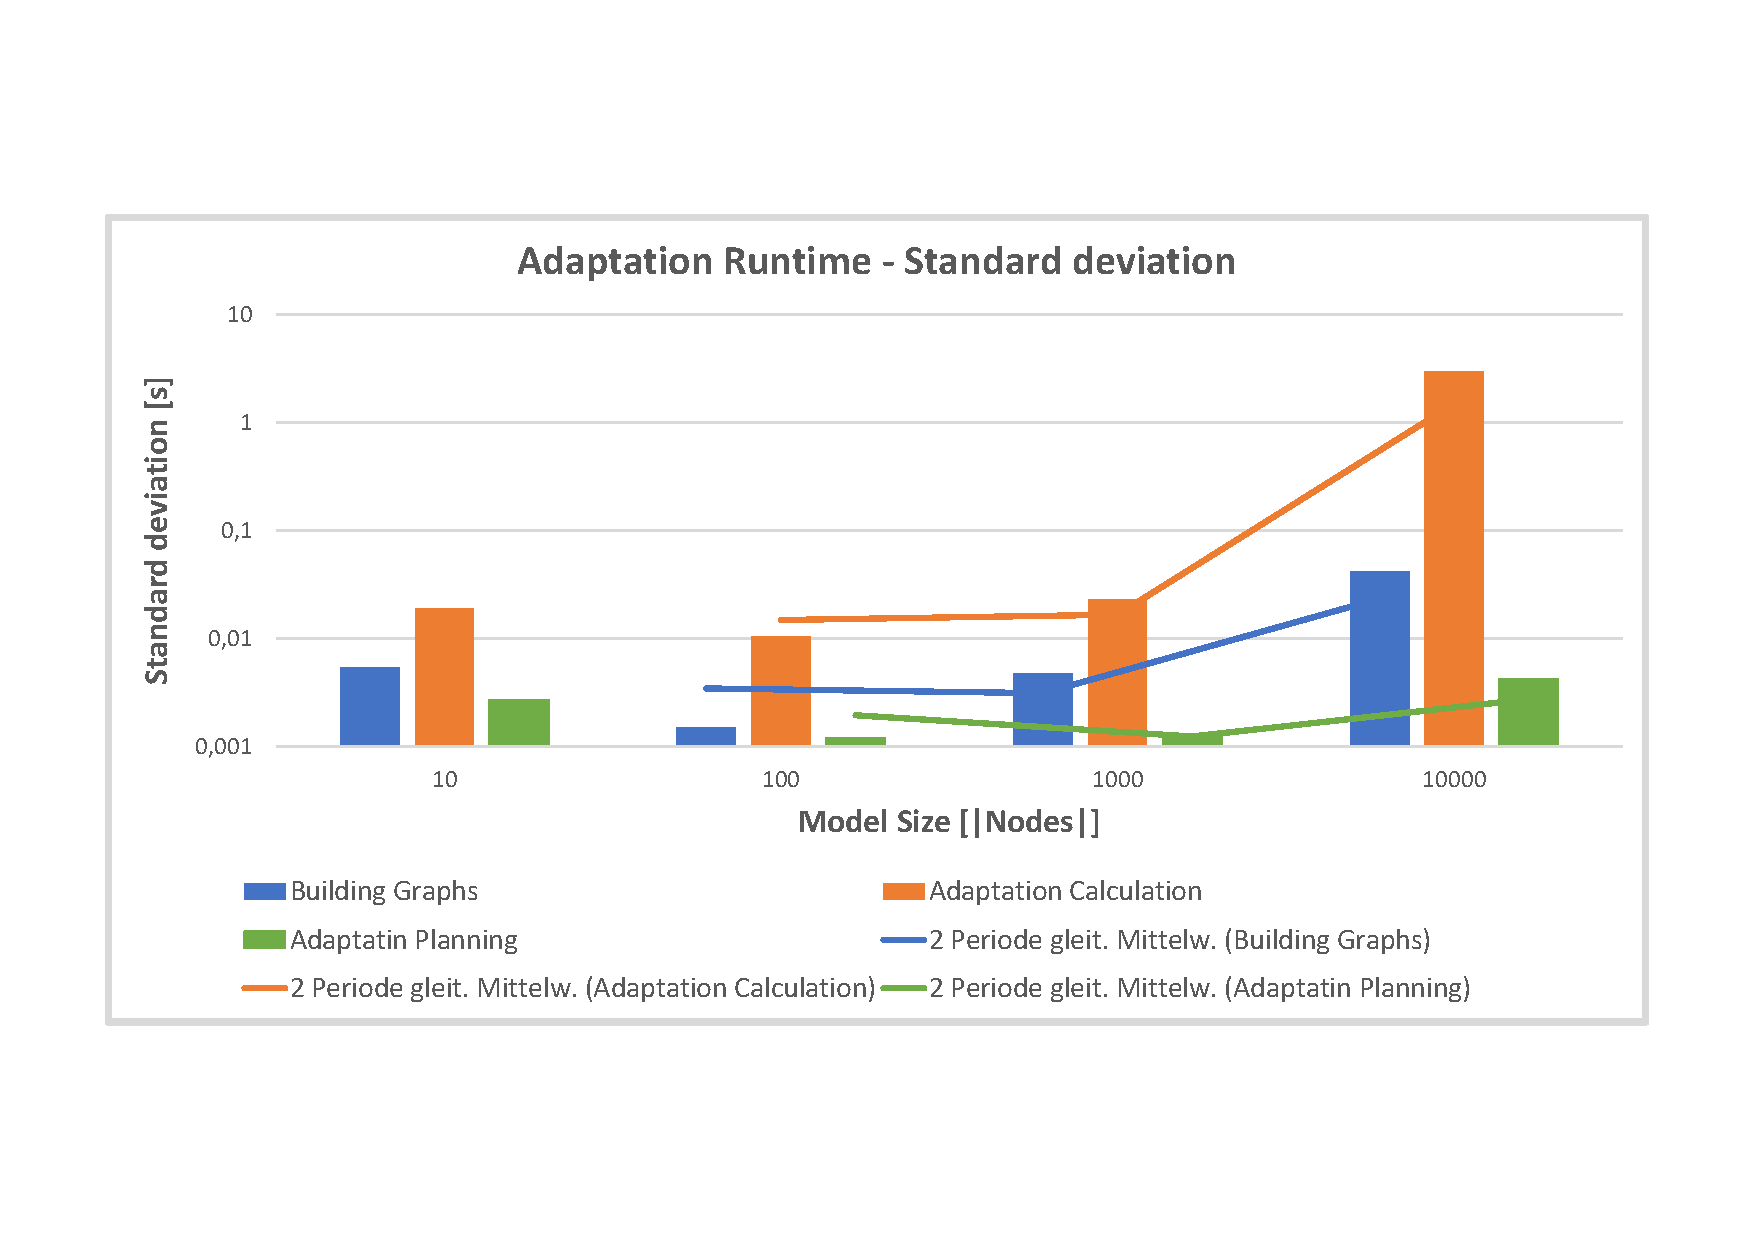
\includegraphics[trim = 10mm 30mm 10mm 20mm, clip, width=0.90\textwidth]{graphs/Runtime_adapt_sd}
	\caption{Adaptation runtime SD}
	\label{fig:eval:adap:runtime_sd}
\end{figure}

\autoref{fig:eval:adap:runtime} shows the runtime results. The graph creation shows a linear runtime behaviour, like in \autoref{sec:Evaluation:privacyanalysis:scale} already noticed. The adaptation calculation consumes an increasingly amount of time. This can be explained with the increasing model size, since the actual action calculation is optimized for $O(1)$ operations, while the action creation operates with PCM model elements directly. The EMF framework in general shows poor performance characteristics, which can also be seen at the failed 100000 changes evaluation \cite{eclipse.org.2009}\cite{Steinberg.20050706}. The adaptation planning needs next to no time, shown by the time line on top of the adaptation calculation line.

The standard deviation (\autoref{fig:eval:adap:runtime_sd}) shows mostly constant deviations. However, the adaptation calculation increases significantly on the last evaluation run. We assume this is due to JVM memory management and EMF effects. However, a standard deviation of roughly 3 seconds to a runtime of 30 seconds is within an acceptable ratio, considering that two models and graphs of 30000 nodes have to be managed.

The \textit{Adaptation Planning} scalability evaluation shows satisfying results. Concerning the research question \textbf{RQ-E3} it is considered very fast with an acceptable variance.


\section{Threats to validity}
\label{sec:eval:threats}

Like in any scientific publications, the evaluation has threats to its validity. We will scope the most important points and highlight the crucial aspects.   

\subsection{Internal Validity} %Cause and Effect

% Accuracy: evaluated every step independently, limited cause and effekt influence => good
Our decision to evaluate every major iObserve Privacy task independently is a key stone to the internal validity. It allowed us to provoke every possible reaction and effect without potential side effects. As a result, we could perfectly track cause and result of certain effects.

% Scalability: Runtime effekts and test-restructuring make test a little "unsharper", however still viable
Scalability tests often require an even more isolated and specialised testing. In our case the individual task had to be called from outside their ordinary call scheme, the \textit{TeeTime framework}. This was necessary so enable tests of the performed size. This blurs the results in the context of the whole system, however, sharpens the individual tasks runtime behaviour.  

\subsection{External Validity} %Generalization

% Used Inputs a Kieker produces => no live tests
One threat towards external validity are the missing live tests. Since testing on a real software system takes way longer, technology specific side effects, dependencies and errors have to be handled, we created inputs by hand. The input is logically and syntactically valid, however, potential corner cases could have been missed, despite extensive testing.  Nevertheless, all tests aiming for a real-world authenticity were using the CoCoME PCM model. This model was designed to provide a scientific comparable, near real-world standard. So, iObserve Privacy was evaluated as close to a real-world application as possible, while using realistic inputs.

% CoCoME is good model, however no real-world model


\subsection{Construction Validity}

% Test every task indepently => minor risk due to well known structure, hand construction of eval models
While the individual task evaluation was the internal validities strength, it is a weakness of the construction validity. However, during the accuracy evaluations, the whole pipeline was (usually) invoked, evaluation scenarios were continued and an internal logically validity was established. So, the evaluation is well interleaved and the likelihood of construction errors should be, despite the individual task evaluation, minimized.

Nevertheless, the target evaluation models are constructed by hand, which tends to be error prone. However, to produce the same error in the evaluation target model like iObserve Privacy does is very unlikely.

\subsection{Conclusion Validity}

% Scalability? bad EMF performance => bad measurement size
The accuracy evaluation is considered very conclusive with sufficient tests, scenarios and models. Most of the scalability evaluations are also quite conclusive. However, the bad EMF performance limits the test sizes. This is especially true for the adaptation planning scalability evaluation, with the maximum input of 10000 changes. This makes the result not as meaning as possible, but still viable.


